%  LaTeX support: latex@mdpi.com
%  For support, please attach all files needed for compiling as well as the log file, and specify your operating system, LaTeX version, and LaTeX editor.

%=================================================================
\documentclass[journal,article,submit,moreauthors]{Definitions/mdpi}

%=================================================================
% MDPI internal commands - do not modify
\firstpage{1}
\makeatletter
\setcounter{page}{\@firstpage}
\makeatother
\pubvolume{1}
\issuenum{1}
\articlenumber{0}
\pubyear{2026}
\copyrightyear{2026}
\datereceived{ }
\daterevised{ }
\dateaccepted{ }
\datepublished{ }

% Compatibilidad entre versiones de la clase MDPI: algunas exigen \hreflink{}.
% Si tu clase no lo define, el \providecommand lo vuelve inofensivo.
\providecommand{\hreflink}[1]{}
\hreflink{https://www.mdpi.com/journal/notspecified}
\providecommand{\isAPAandChicago}[2]{#2}

%=================================================================
% Full title of the paper (Capitalized)
\Title{An Edge–Fog–Cloud Architectural Framework for Distributed IoT Intrusion Detection Based on Hierarchical Federated Learning}

% Author ORCID ID: enter ID or remove command
\newcommand{\orcidauthorA}{0000-0003-2920-6320} % Add \orcidA{} behind the author's name

% Authors, for the paper (add full first names)
\Author{Santiago Jaimes $^{1}$, Nicolas Casas $^{1}$ and Carlos Lozano-Garzon $^{1}$\orcidA{}}

% MDPI internal command: Authors, for metadata in PDF
\AuthorNames{Santiago Jaimes, Nicolas Casas and Carlos Lozano-Garzon}

% Affiliations / Addresses (Add [1] after \address if there is only one affiliation.)
\address{%
$^{1}$ \quad Systems and Computing Engineering Department, Universidad de los Andes, Bogota, 111711, Colombia}

% Contact information of the corresponding author
\corres{Correspondence: e-mail@uniandes.edu.co}

% Abstract (Do not insert blank lines, i.e. \\)
\abstract{Distributed intrusion detection systems have become an effective approach for protecting Internet of Things (IoT) environments, where the computational constraints of Edge devices, data distribution, and privacy requirements limit the applicability of traditional centralized security solutions. Although recent research has explored TinyML, federated learning, and lightweight cryptography as enabling technologies for IoT security, most existing approaches examine these capabilities in isolation, offering limited evidence of their behavior when integrated into a unified distributed architecture. This paper presents an Edge--Fog--Cloud architecture for distributed intrusion detection in IoT environments that integrates TinyML-based inference, hierarchical federated learning, and secure communications into a unified architectural framework. The proposed architecture is validated through a comprehensive experimental design that jointly evaluates five complementary dimensions: detection capability, collaborative learning behavior, deployment feasibility on resource-constrained Edge devices, operational efficiency, and the impact of communication security mechanisms. The experimental results show that the proposed architecture maintains consistent detection performance, preserves the stability of hierarchical federated learning, supports deployment on resource-constrained platforms, and incorporates secure communications with limited operational overhead. Furthermore, the experimental evidence indicates that the overall system behavior is determined by the interaction among its architectural components rather than by the isolated optimization of individual technologies. Beyond validating a distributed intrusion detection architecture for IoT, this work proposes an architectural design framework for future Edge--Fog--Cloud security systems. The results show that integrating Edge intelligence, collaborative learning, and secure communications provides a practical foundation for developing distributed intrusion detection systems that address scalability, computational efficiency, privacy, and security in IoT ecosystems.}

% Keywords
\keyword{Distributed Intrusion Detection; Internet of Things; Edge--Fog--Cloud Architecture; Hierarchical Federated Learning; TinyML; Lightweight Cryptography.}

%%%%%%%%%%%%%%%%%%%%%%%%%%%%%%%%%%%%%%%%%%
\begin{document}

%%%%%%%%%%%%%%%%%%%%%%%%%%%%%%%%%%%%%%%%%%

\section{Introduction}

El crecimiento acelerado del Internet de las Cosas (IoT) y del Internet Industrial de las Cosas (IIoT) ha impulsado el despliegue de millones de dispositivos conectados en sectores como la manufactura, la energía, la salud y las ciudades inteligentes. Aunque esta transformación ha ampliado significativamente las capacidades de monitoreo y automatización, también ha incrementado la superficie de ataque de las infraestructuras distribuidas, exponiendo dispositivos con recursos limitados a un número creciente de amenazas cibernéticas. En este contexto, los sistemas de detección de intrusiones (Intrusion Detection Systems, IDS) se han convertido en un componente fundamental para identificar comportamientos anómalos y fortalecer la resiliencia de las redes IoT frente a ataques cada vez más sofisticados \cite{Ni2024,Amanullah2020,Bagaa2020}. Las revisiones sistemáticas más recientes del panorama de seguridad en IoT coinciden en que esta superficie de ataque ya no puede caracterizarse únicamente a partir de vulnerabilidades individuales de los dispositivos, sino a partir de la arquitectura que los interconecta: es la combinación de protocolos ligeros, capacidad de cómputo escasa y despliegues heterogéneos la que determina qué mecanismos de defensa resultan viables en cada nivel de la infraestructura \cite{Lim2025}.

Los enfoques tradicionales para la detección de intrusiones fueron concebidos para operar en infraestructuras centralizadas con abundantes recursos computacionales. Sin embargo, las restricciones de memoria, capacidad de procesamiento, consumo energético y conectividad, propias de los dispositivos IoT, dificultan la adopción directa de estos mecanismos en el borde de la red. Como consecuencia, la arquitectura de los IDS ha evolucionado progresivamente hacia esquemas distribuidos capaces de realizar inferencia local, reducir la latencia de detección y disminuir la dependencia de conexiones permanentes con la nube. Este cambio ha consolidado las arquitecturas Edge--Fog--Cloud como una alternativa para distribuir las funciones de procesamiento según las capacidades disponibles en cada nivel de la infraestructura \cite{SaravanaBalaji2023,Ni2024,Dini2024}. Las revisiones sistemáticas sobre detección de intrusiones en entornos \textit{Fog} confirman este desplazamiento: el nivel intermedio concentra hoy buena parte de las funciones de seguridad que anteriormente residían en la nube, precisamente porque combina la proximidad a los dispositivos con recursos computacionales superiores a los disponibles en el borde \cite{Tamuka2026}.

La evolución hacia arquitecturas distribuidas ha impulsado el desarrollo de tecnologías complementarias que abordan distintos desafíos del problema. TinyML permite ejecutar modelos compactos directamente sobre microcontroladores; el aprendizaje federado posibilita la actualización colaborativa de dichos modelos sin centralizar los datos utilizados para el entrenamiento; y la criptografía ligera proporciona mecanismos eficientes para proteger las comunicaciones en dispositivos con recursos restringidos \cite{Tekin2023,Amuthadevi2025,McMahan2017,Imteaj2022,NIST800232,Kaur2025}. En conjunto, estas tecnologías constituyen los pilares para el desarrollo de sistemas inteligentes capaces de operar de manera distribuida, eficiente y segura.

No obstante, la integración de estas capacidades plantea nuevos desafíos arquitectónicos. La inferencia distribuida requiere modelos compatibles con las restricciones del hardware embebido; el entrenamiento colaborativo incorpora nuevos flujos de comunicación y modifica la organización funcional del sistema; y la protección criptográfica debe garantizar la confidencialidad, la integridad y la autenticidad de las actualizaciones intercambiadas sin comprometer el desempeño global de la arquitectura. En consecuencia, la evaluación de estas tecnologías de manera independiente resulta insuficiente para comprender el comportamiento de un IDS distribuido cuando todos estos componentes interactúan dentro de una misma infraestructura. Las propuestas que abordan explícitamente esta convergencia entre inteligencia distribuida, aprendizaje colaborativo y protección de las comunicaciones comienzan a aparecer en la literatura más reciente, pero su validación se apoya predominantemente en conjuntos de datos de referencia ejecutados sobre infraestructura convencional, lo que deja abierta la caracterización del comportamiento de estos sistemas cuando operan sobre dispositivos reales \cite{Alshammari2026,Dritsas2025}.

Con el propósito de contribuir a la solución de este problema, este trabajo presenta una arquitectura integrada Edge--Fog--Cloud para la detección distribuida de intrusiones en redes IoT/MQTT que combina inferencia TinyML en nodos ESP32-S3, aprendizaje federado jerárquico mediante gateways Raspberry Pi 4 y protección criptográfica basada en ASCON-128 para asegurar el intercambio de parámetros durante el entrenamiento colaborativo. La propuesta se implementa íntegramente en hardware real y se evalúa considerando diferentes configuraciones arquitectónicas, variantes de modelos compactos y mecanismos de agregación federada, lo que permite analizar conjuntamente el desempeño del sistema desde la perspectiva de la precisión de detección, la eficiencia computacional, el costo de comunicación y la sobrecarga introducida por los mecanismos criptográficos. Más allá del desempeño alcanzado por un modelo específico, la principal contribución del trabajo consiste en demostrar la viabilidad de integrar estas tecnologías en una arquitectura Edge--Fog--Cloud funcional y en cuantificar experimentalmente los beneficios, compromisos y limitaciones que emergen cuando se evalúan como un sistema unificado.

%%%%%%%%%%%%%%%%%%%%%%%%%%%%%%%%%%%%%%%%%%
\section{Related Works}
\label{related}

El diseño de sistemas de detección de intrusiones para Internet de las Cosas ha evolucionado en respuesta a una serie de desafíos impuestos por la naturaleza distribuida de estos entornos, las limitaciones computacionales de los dispositivos y la necesidad de mantener mecanismos de detección capaces de adaptarse a amenazas en constante evolución. Como resultado, la investigación reciente ha generado diversas soluciones para abordar problemas específicos relacionados con la ejecución de modelos de aprendizaje, su actualización continua y la protección de la información intercambiada durante dicho proceso. Más que representar desarrollos aislados, estos avances constituyen decisiones arquitectónicas complementarias que, en conjunto, determinan la viabilidad de un IDS distribuido en entornos IoT.

Desde esta perspectiva, la presente revisión organiza el estado del arte en función de la evolución funcional de una arquitectura Edge--Fog--Cloud. En primer lugar, se analizan los avances en TinyML como mecanismo para trasladar la inferencia a dispositivos con recursos limitados. Posteriormente, se revisa el aprendizaje federado como estrategia para mantener modelos distribuidos mediante entrenamiento colaborativo sin centralizar los datos. A continuación, se estudia el papel de la criptografía ligera en la protección de las comunicaciones y del conocimiento intercambiado durante dicho proceso. Finalmente, estas tres líneas de investigación convergen en la identificación de la brecha científica y experimental que fundamenta la propuesta presentada en este artículo.

\subsection{TinyML-Based Intrusion Detection for IoT}
La evolución de los sistemas de detección de intrusiones (IDS) para el Internet de las Cosas ha estado estrechamente ligada a la transformación de las arquitecturas de procesamiento. Mientras que las primeras soluciones fueron concebidas para operar en servidores o infraestructuras centralizadas con amplios recursos computacionales, el crecimiento del número de dispositivos IoT y IIoT, junto con sus restricciones de memoria, capacidad de procesamiento, consumo energético y conectividad, evidenció la necesidad de trasladar progresivamente las capacidades de detección a los nodos de borde. Este cambio de paradigma respondió no solo a la necesidad de reducir la latencia de respuesta y el consumo de ancho de banda, sino también a la creciente demanda de sistemas capaces de operar de manera autónoma y distribuida en entornos altamente dinámicos \cite{Ni2024,Amanullah2020,Bagaa2020,SaravanaBalaji2023}. Esta evolución no ha sido lineal: la literatura reciente muestra que el desplazamiento de las funciones de detección hacia el borde se ha producido de forma escalonada, apoyándose en niveles intermedios que asumen las tareas que los dispositivos más limitados no pueden ejecutar, de modo que la capacidad de detección termina distribuida entre varios niveles en lugar de residir en uno solo \cite{Tamuka2026}.

En este contexto, TinyML se consolidó como una estrategia para ejecutar modelos de aprendizaje automático directamente en microcontroladores y otros dispositivos con recursos limitados. Más que una nueva familia de algoritmos, TinyML representa un cambio en la forma de diseñar soluciones inteligentes para el borde, combinando modelos compactos, técnicas de optimización y herramientas de despliegue que permiten realizar inferencia local dentro de las limitaciones del hardware embebido. Como resultado, la detección de intrusiones dejó de depender exclusivamente de plataformas centralizadas y comenzó a integrarse como una capacidad propia de los dispositivos IoT, lo que permitió tiempos de respuesta más reducidos y una mayor resiliencia frente a interrupciones de conectividad \cite{Tekin2023,Amuthadevi2025,Dini2024,Heydari2024}.

La consolidación de TinyML también modificó la forma en que se evalúan los sistemas de detección de intrusiones en IoT. Si bien la precisión continúa siendo un indicador fundamental, la literatura reciente reconoce que métricas como la huella de memoria, la latencia de inferencia, el consumo energético y la factibilidad de despliegue son igualmente determinantes para evaluar la viabilidad operativa de un modelo en plataformas embebidas. En consecuencia, la evaluación de los IDS ha evolucionado desde una perspectiva centrada exclusivamente en el desempeño del clasificador hacia un análisis integral que considera simultáneamente el costo computacional y las restricciones del entorno de ejecución \cite{Tekin2023,Amuthadevi2025,Dini2024,Heydari2024}. Los trabajos de referencia sobre evaluación comparativa de sistemas TinyML han formalizado este conjunto ampliado de indicadores y proponen metodologías específicas para medir conjuntamente la exactitud, la latencia, la huella de memoria y el consumo energético, subrayando que estas magnitudes deben obtenerse sobre la plataforma de destino y no estimarse a partir del modelo entrenado \cite{HeydariSurvey2025,Bartoli2025,Banbury2020}.

No obstante, la capacidad de realizar inferencia local constituye únicamente una parte del ciclo de vida de un IDS inteligente. En escenarios operativos, los modelos deben actualizarse para incorporar nuevos patrones de tráfico, adaptarse a cambios en el comportamiento de la red y responder a amenazas emergentes. Sin embargo, la mayor parte de las investigaciones continúa concentrándose en la inferencia sobre dispositivos Edge, mientras que el entrenamiento y la actualización de los modelos suelen permanecer centralizados o realizarse en plataformas con recursos considerablemente superiores a los disponibles en microcontroladores \cite{Ficco2024,Ramadan2025}. Las investigaciones orientadas al aprendizaje continuo sobre el propio dispositivo abordan directamente esta asimetría y muestran que un microcontrolador puede incorporar actualizaciones del modelo durante su operación, siempre que el procedimiento de actualización se diseñe bajo las mismas restricciones de memoria y de cómputo que gobiernan la inferencia \cite{Ren2024}.

En consecuencia, el desafío actual ya no consiste únicamente en demostrar que un modelo puede ejecutarse sobre hardware restringido, sino en mantener su capacidad de adaptación sin perder las ventajas derivadas del procesamiento distribuido. Esta necesidad ha impulsado la incorporación del aprendizaje federado como alternativa para extender el ciclo de vida de los modelos más allá de la inferencia local, permitiendo que múltiples dispositivos colaboren en el proceso de entrenamiento sin compartir directamente sus datos. Desde esta perspectiva, el aprendizaje federado representa una evolución natural del paradigma TinyML y constituye el siguiente paso hacia arquitecturas de detección de intrusiones verdaderamente distribuidas.

\subsection{Federated Learning for Distributed Intrusion Detection}
El desplazamiento de la inferencia hacia los dispositivos de borde resolvió parcialmente las limitaciones asociadas a la latencia, el consumo de ancho de banda y la dependencia de infraestructuras centralizadas. Sin embargo, esta evolución trasladó el principal desafío de la ejecución del modelo al mantenimiento. A diferencia de los entornos tradicionales, donde los modelos pueden entrenarse periódicamente a partir de un repositorio centralizado de datos, las redes IoT generan información de forma continua, distribuida y altamente heterogénea. Los cambios en los patrones de tráfico, la incorporación de nuevos dispositivos y la aparición constante de amenazas hacen que un modelo estático pierda progresivamente su capacidad de detección. En consecuencia, la adaptación continua del conocimiento se convirtió en un requisito fundamental para los IDS distribuidos, dando origen a una nueva línea de investigación centrada en mecanismos de entrenamiento colaborativo capaces de operar directamente sobre infraestructuras Edge \cite{McMahan2017,Imteaj2022,Ramadan2025}. La necesidad de adaptación continua no se limita al ámbito de la ciberseguridad: los trabajos sobre gestión y actualización de sistemas TinyML desplegados muestran que mantener vigente un modelo exige mecanismos explícitos de aprendizaje en línea, sin los cuales el conocimiento embebido en el dispositivo queda congelado en el momento del despliegue \cite{Ren2024}.

El aprendizaje federado surgió como respuesta a este desafío al permitir que múltiples participantes colaboren en el entrenamiento de un modelo compartido sin necesidad de transferir sus datos originales. En este paradigma, cada nodo actualiza localmente el modelo utilizando la información disponible en su entorno y transmite únicamente los parámetros aprendidos a un coordinador responsable de construir un modelo global. Esta estrategia reduce la transferencia de información sensible, preserva la privacidad de los datos locales y disminuye la dependencia de infraestructuras centralizadas, características especialmente relevantes para aplicaciones de ciberseguridad en las que los datos monitoreados pueden contener información crítica sobre la operación de la red \cite{McMahan2017,Imteaj2022,Hajj2023,Roy2023}.

La incorporación del aprendizaje federado modificó la forma en que se diseñan y se evalúan los IDS distribuidos. La atención dejó de centrarse exclusivamente en el desempeño del clasificador para incorporar aspectos propios del proceso colaborativo de entrenamiento, como el costo de la comunicación entre participantes, la frecuencia de sincronización, la convergencia del aprendizaje y el comportamiento frente a distribuciones de datos heterogéneas (non-IID). Estos factores han demostrado que el desempeño global del sistema depende tanto del modelo de aprendizaje como de la arquitectura de comunicación que sustenta el proceso colaborativo, especialmente en despliegues IoT, donde la conectividad, la disponibilidad de recursos y la distribución del tráfico presentan un elevado grado de variabilidad \cite{Imteaj2022,Hajj2023,Chaurasia2024,Albanbay2025,Ramadan2025}. Las evaluaciones experimentales de esquemas federados organizados por niveles muestran que la frecuencia de sincronización y la ruta que siguen las actualizaciones condicionan de manera directa el número de rondas necesarias para alcanzar un modelo estable, lo que convierte la topología de comunicación en un parámetro de diseño equiparable a los hiperparámetros del propio entrenamiento \cite{Ma2024,Cooray2025}.

A medida que el número de participantes aumenta, el proceso de sincronización también se convierte en un factor determinante para la escalabilidad del sistema. Como respuesta, la literatura ha evolucionado desde esquemas convencionales de aprendizaje federado hacia arquitecturas jerárquicas en las que los nodos intermedios realizan procesos de agregación antes de sincronizar el modelo con el coordinador global. Más allá de representar una optimización del algoritmo FedAvg, estas arquitecturas redefinen la organización funcional del sistema al distribuir responsabilidades entre los niveles Edge, Fog y Cloud, reduciendo el tráfico de comunicaciones y aproximando el proceso de entrenamiento a la estructura propia de las infraestructuras IoT de gran escala \cite{Ficco2024,Tran2026,Ramadan2025}. Los estudios que comparan directamente ambas organizaciones reportan que la agregación intermedia reduce el número de actualizaciones que alcanzan al coordinador global y acorta la distancia de comunicación de la mayoría de los mensajes, aunque introduce un nivel adicional de coordinación cuyo costo debe contabilizarse al evaluar el beneficio neto \cite{Ma2024,Cooray2025}.

Aunque el aprendizaje federado evita compartir directamente los datos utilizados durante el entrenamiento, las actualizaciones del modelo intercambiadas entre los participantes constituyen un nuevo activo crítico en la arquitectura. Diversos estudios han señalado que estos parámetros pueden revelar información sobre los datos locales, ser manipulados para degradar el proceso de aprendizaje o convertirse en un vector para ataques dirigidos contra el modelo global \cite{Imteaj2022,Hajj2023}. Las revisiones dedicadas específicamente al aprendizaje federado con preservación de la privacidad en sistemas de detección de intrusiones agrupan estas amenazas en dos familias: las que buscan reconstruir información sobre los datos locales a partir de los parámetros intercambiados y las que persiguen degradar el modelo global mediante actualizaciones manipuladas. Ambas persisten aunque el canal de comunicación se encuentre cifrado, ya que se originan en el contenido de las contribuciones y no en su transporte \cite{Bunko2026}.

En consecuencia, la evolución del aprendizaje federado no solo ha transformado la manera en que los IDS distribuidos actualizan sus modelos, sino que también ha incorporado nuevos requisitos de seguridad asociados a la protección del conocimiento intercambiado durante el entrenamiento colaborativo. Bajo esta perspectiva, garantizar la confidencialidad, la integridad y la autenticidad de las actualizaciones del modelo constituye un requisito arquitectónico tan importante como el propio mecanismo de aprendizaje, lo que motiva la incorporación de esquemas de criptografía ligera capaces de operar dentro de las restricciones propias de los dispositivos IoT.

\subsection{Lightweight Cryptography for Trustworthy Distributed Learning}
La evolución de los IDS hacia arquitecturas distribuidas ha modificado progresivamente la naturaleza de los activos que deben protegerse. En los enfoques tradicionales, la seguridad se concentraba principalmente en preservar la confidencialidad e integridad del tráfico de red, las credenciales de acceso y la información almacenada en los dispositivos. Sin embargo, cuando el entrenamiento pasa a realizarse de manera colaborativa, el conocimiento generado por el sistema adquiere un valor estratégico. Las actualizaciones del modelo, los parámetros intercambiados durante las rondas federadas y los mensajes de sincronización dejan de ser simples datos de control para convertirse en elementos esenciales para el funcionamiento del IDS. Como consecuencia, proteger el proceso de aprendizaje pasa a ser tan importante como proteger el tráfico inspeccionado por el propio sistema. Esta reorientación del activo que debe protegerse está ampliamente documentada: la literatura sobre confiabilidad en aprendizaje federado sitúa los parámetros intercambiados como el elemento central del sistema y distingue entre protegerlos frente a observadores externos, mediante mecanismos criptográficos, y protegerlos frente a los propios participantes, lo que exige garantías de naturaleza distinta \cite{Bunko2026,Alshammari2026}.

Las restricciones computacionales de los dispositivos IoT hacen que la protección de este nuevo activo requiera mecanismos distintos de los empleados tradicionalmente en infraestructuras de mayor capacidad. Aunque las soluciones criptográficas convencionales ofrecen altos niveles de seguridad, su implementación puede introducir costos incompatibles con las limitaciones de memoria, de procesamiento y de consumo energético propias de microcontroladores y plataformas Edge. Estas condiciones impulsaron el desarrollo de algoritmos de criptografía ligera capaces de preservar la confidencialidad, la integridad y la autenticidad de la información, manteniendo un costo computacional reducido \cite{NISTIR8454,NIST800232,Gusita2025,Kaur2025}. Los análisis comparativos de estos algoritmos sobre plataformas IoT con recursos restringidos muestran que las diferencias de desempeño entre candidatos dependen fuertemente de la plataforma de destino y del tamaño de los mensajes procesados, por lo que la elección de un esquema concreto no puede desligarse del perfil de tráfico de la aplicación \cite{Sorescu2025}.

La estandarización de ASCON por parte del National Institute of Standards and Technology (NIST) representa la consolidación de esta línea de investigación y proporciona un mecanismo ampliamente aceptado para proteger aplicaciones desplegadas en dispositivos con recursos restringidos. Además de sus propiedades criptográficas, la disponibilidad de un estándar abierto favorece la interoperabilidad entre implementaciones y facilita la incorporación de mecanismos de protección en arquitecturas IoT heterogéneas \cite{NIST800232,Kaur2025}.

La literatura reciente ha estudiado ampliamente el desempeño de algoritmos de criptografía ligera, su implementación en plataformas embebidas y su resistencia frente a diferentes vectores de ataque, incluidos ataques de canal lateral, inyección de fallas y debilidades asociadas con construcciones criptográficas ultraligeras \cite{Kaur2025,Mirzaali2025,Gusita2025}. Sin embargo, la mayoría de estas investigaciones evalúa los mecanismos criptográficos como componentes independientes o dentro de aplicaciones específicas, sin analizar explícitamente su interacción con procesos de aprendizaje distribuido ejecutados en arquitecturas Edge--Fog--Cloud.

Un caso reciente ilustra tanto el interés como los límites actuales de esta línea. Alshammari \cite{Alshammari2026} propone un marco unificado que combina detección de intrusiones eficiente en energía, criptografía ligera basada en ASCON y aprendizaje federado jerárquico sobre una organización Edge--Fog--Cloud, cuantificando el ahorro energético y la reducción de emisiones asociadas al proceso. No obstante, su validación se apoya en conjuntos de datos de referencia evaluados sobre infraestructura convencional, por lo que el costo real de las operaciones criptográficas y del ciclo federado sobre microcontroladores permanece sin caracterizar experimentalmente. Este caso ilustra además una carencia metodológica más general: los esquemas de cifrado autenticado suelen incorporarse como un servicio externo al proceso de aprendizaje, de modo que su costo se reporta de forma agregada y no resulta posible atribuirlo a las etapas concretas del ciclo federado ni a los canales que lo componen.

En consecuencia, aunque la criptografía ligera constituye hoy un componente esencial para proteger las aplicaciones IoT, continúa existiendo evidencia limitada sobre el impacto que estos mecanismos generan cuando forman parte del ciclo completo de aprendizaje distribuido. Aspectos como el costo temporal del cifrado \cite{Sorescu2025}, el incremento del tráfico asociado al intercambio de modelos, su influencia en la sincronización entre participantes y el efecto en la convergencia del entrenamiento permanecen insuficientemente caracterizados en arquitecturas completas ejecutadas en hardware restringido. Esta situación sugiere que la protección criptográfica no debe analizarse como un componente independiente, sino como un requisito arquitectónico cuya evaluación debe integrarse con la inferencia en el borde y el aprendizaje colaborativo. La distinción es relevante en términos prácticos: el costo de una operación criptográfica aislada puede medirse sobre un microcontrolador mediante un banco de pruebas sencillo, mientras que su efecto acumulado a lo largo de una ronda federada depende del número de mensajes intercambiados, de su tamaño y del nivel de la arquitectura en el que se ejecuta cada operación, magnitudes que solo emergen al instrumentar el ciclo completo \cite{Alshammari2026}.

\subsection{Research Gap and Motivation}
La literatura revisada evidencia un avance significativo en tres líneas de investigación que han contribuido a la evolución de los sistemas de detección de intrusiones en IoT. Por una parte, TinyML ha demostrado la viabilidad de ejecutar modelos de aprendizaje automático directamente en dispositivos con recursos limitados, acercando la capacidad de inferencia al borde de la red y reduciendo la dependencia de infraestructuras centralizadas \cite{Tekin2023,Amuthadevi2025,Dini2024}. Paralelamente, el aprendizaje federado ha permitido mantener modelos distribuidos mediante entrenamiento colaborativo, sin necesidad de centralizar los datos utilizados por cada participante, lo que favorece arquitecturas más escalables y respetuosas de la privacidad \cite{McMahan2017,Imteaj2022,Hajj2023,Ramadan2025}. Finalmente, la criptografía ligera ha proporcionado mecanismos eficientes para proteger las comunicaciones y la información intercambiada entre dispositivos con recursos limitados, consolidándose como un componente fundamental para el desarrollo de aplicaciones IoT seguras \cite{NIST800232,Kaur2025,Gusita2025}.

A pesar de estos avances, las tres líneas de investigación han evolucionado principalmente de forma independiente. Los trabajos orientados a TinyML se concentran en optimizar la inferencia en hardware restringido; las investigaciones sobre aprendizaje federado analizan el comportamiento de los algoritmos de entrenamiento distribuido y sus mecanismos de agregación; mientras que la literatura sobre criptografía ligera estudia el desempeño y la robustez de los algoritmos criptográficos en plataformas embebidas. Existen ya propuestas que combinan varios de estos componentes dentro de una misma arquitectura. Alshammari \cite{Alshammari2026} integra detección de intrusiones, criptografía ligera ASCON y aprendizaje federado jerárquico en una organización Edge--Fog--Cloud; Tran et al. \cite{Tran2026} incorporan agregación jerárquica y mecanismos criptográficos sobre plataformas embebidas; y Ramadan et al. \cite{Ramadan2025} sistematizan las prácticas actuales de aprendizaje federado con TinyML en dispositivos de borde. Sin embargo, estas propuestas se evalúan predominantemente sobre conjuntos de datos de referencia o infraestructuras convencionales, de manera que la caracterización experimental del comportamiento conjunto de las tres tecnologías --- medida extremo a extremo sobre microcontroladores reales, con instrumentación por canal de comunicación y por ronda federada --- continúa siendo limitada. En particular, no se dispone de mediciones que asocien el costo de cada operación criptográfica al canal y al nivel arquitectónico en el que se ejecuta, ni de series temporales que permitan verificar si ese costo permanece estable a lo largo de las rondas sucesivas de entrenamiento. Es precisamente en esa evidencia empírica, y no en la propuesta de un nuevo algoritmo, donde se sitúa la contribución de este trabajo.

Esta limitación no es únicamente tecnológica, sino también metodológica. La mayor parte de la literatura evalúa de forma aislada el desempeño de los modelos de aprendizaje, la eficiencia de los algoritmos de agregación o las propiedades de los mecanismos criptográficos. En consecuencia, aspectos como la interacción entre estos componentes, el costo conjunto de su integración, el impacto en la comunicación entre niveles arquitectónicos y los compromisos entre la precisión de detección, la eficiencia computacional, la sobrecarga criptográfica y la escalabilidad permanecen insuficientemente caracterizados. Desde la perspectiva del diseño de sistemas, comprender estas interacciones es esencial para determinar la viabilidad de arquitecturas distribuidas destinadas a escenarios de IoT reales. El problema de fondo es que cada uno de estos compromisos se ha estudiado en un plano distinto: la exactitud frente al tamaño del modelo en la literatura de TinyML, el costo de comunicación frente a la velocidad de convergencia en la de aprendizaje federado, y el nivel de protección frente al consumo de recursos en la de criptografía ligera. Sin una medición conjunta resulta imposible determinar si las mejoras obtenidas en una de estas dimensiones se sostienen cuando las tres operan simultáneamente \cite{Alshammari2026,Cooray2025}.

En este contexto, el presente trabajo propone una arquitectura integrada Edge--Fog--Cloud que combina inferencia TinyML en nodos ESP32-S3, aprendizaje federado jerárquico mediante gateways Raspberry Pi 4 y protección criptográfica basada en ASCON-128 para asegurar las comunicaciones durante el ciclo de entrenamiento colaborativo. A diferencia de enfoques orientados al desarrollo de un nuevo algoritmo de aprendizaje o de un nuevo mecanismo criptográfico, esta investigación se centra en la caracterización experimental de la arquitectura como un sistema unificado. Para ello, se analizan conjuntamente diferentes configuraciones de aprendizaje, mecanismos de agregación y esquemas de protección criptográfica, cuantificando su impacto en la precisión de detección, el costo computacional, la comunicación entre participantes y la sobrecarga introducida por los mecanismos de seguridad. De esta manera, el trabajo contribuye a una mejor comprensión de los compromisos de diseño que emergen cuando la inferencia distribuida, el aprendizaje colaborativo y la protección criptográfica coexisten en una misma arquitectura IoT implementada en hardware con recursos restringidos.

%%%%%%%%%%%%%%%%%%%%%%%%%%%%%%%%%%%%%%%%%%
\section{Proposed Architecture}
\label{sec:architecture}

La integración de mecanismos de detección de intrusiones, aprendizaje federado y criptografía ligera requiere una arquitectura que permita aprovechar las capacidades de cada uno de estos componentes sin trasladar innecesariamente la complejidad computacional a los dispositivos IoT. Mientras la inferencia demanda respuestas de baja latencia cercanas al origen de los datos, el entrenamiento colaborativo y la coordinación del modelo requieren más recursos de procesamiento y una visión global del sistema. Al mismo tiempo, el intercambio continuo de información en el aprendizaje distribuido introduce nuevos requerimientos de protección que deben abordarse sin comprometer la eficiencia operativa de la infraestructura.

Para responder a estas necesidades, se propone una arquitectura jerárquica basada en el paradigma \textit{Edge--Fog--Cloud}, en la que las responsabilidades del sistema se distribuyen de acuerdo con las capacidades computacionales y funcionales de cada nivel. Esta organización permite desacoplar la inferencia en tiempo real del proceso de aprendizaje colaborativo, preservar el carácter distribuido del entrenamiento y facilitar la integración de mecanismos de seguridad en los canales de comunicación sin modificar la dinámica general del sistema. Como resultado, la arquitectura establece un marco unificado para la generación, consolidación y protección del conocimiento distribuido, lo que permite que el modelo evolucione continuamente a partir de la experiencia adquirida en los diferentes dominios de operación.

\subsection{Architectural Overview}
La arquitectura propuesta fue diseñada para integrar inferencia distribuida, aprendizaje colaborativo y mecanismos de protección criptográfica en un único flujo operativo para la detección de intrusiones en entornos IoT. En lugar de considerar estas capacidades como componentes independientes, la propuesta las organiza como partes de un mismo sistema, distribuyendo sus responsabilidades de acuerdo con los requisitos de latencia, capacidad de procesamiento y comunicación propios de cada etapa del proceso. Este enfoque permite que las tareas críticas para la detección permanezcan próximas al origen de los datos, mientras que las funciones de entrenamiento y coordinación se ejecutan en niveles de infraestructura con mayores recursos computacionales, siguiendo los principios de las arquitecturas \textit{Edge--Fog--Cloud} \cite{SaravanaBalaji2023,Wang2019,Ficco2024}.

La arquitectura adopta una organización jerárquica compuesta por tres niveles funcionales: \textit{Edge}, \textit{Fog} y \textit{Cloud}, cada uno especializado en un conjunto de responsabilidades a lo largo del ciclo completo de detección y aprendizaje. Esta distribución funcional evita concentrar toda la carga computacional en un único nivel de la infraestructura y permite equilibrar la eficiencia, la escalabilidad y la capacidad de respuesta. La Figura~\ref{fig:architecture} presenta la organización general de la arquitectura, mientras que la Tabla~\ref{tab:architecture_roles} sintetiza el objetivo arquitectónico y la contribución de cada nivel al proceso de aprendizaje distribuido.

\begin{figure}[ht]
    \centering
    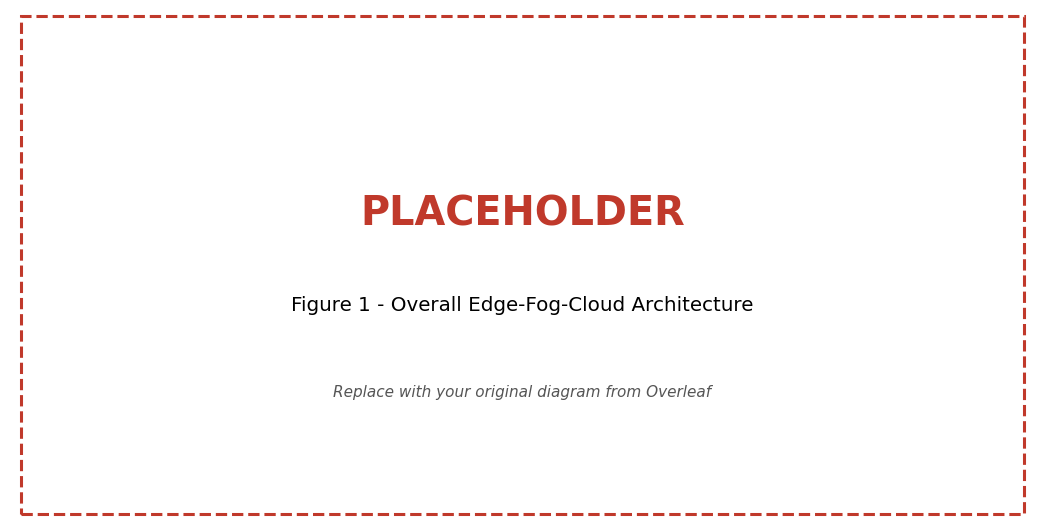
\includegraphics[width=\linewidth]{Figures/architecture.png}
    \caption{Overall architecture of the proposed Edge--Fog--Cloud intrusion detection system.}
    \label{fig:architecture}
\end{figure}

\begin{table}[t]
\centering
\caption{Contribución de cada nivel al ciclo de aprendizaje distribuido de la arquitectura propuesta.}
\label{tab:architecture_roles}
\renewcommand{\arraystretch}{1.25}
\footnotesize
\begin{tabular}{l p{3cm}p{3.5cm}p{5cm}}
\toprule
\textbf{Nivel} & \textbf{Objetivo arquitectónico} & \textbf{Contribución al aprendizaje} & \textbf{Justificación de diseño} \\
\midrule
\textit{Edge} & Detección local en tiempo real. & Genera las observaciones locales utilizadas durante el aprendizaje. & Reduce la latencia, evita la transmisión continua del tráfico y mantiene la operación del IDS en dispositivos con recursos limitados. \\
\textit{Fog} & Aprendizaje colaborativo distribuido. & Transforma las observaciones locales en actualizaciones del modelo. & Desacopla la inferencia del entrenamiento y preserva la privacidad de los datos utilizados durante el aprendizaje. \\
\textit{Cloud} & Coordinación global del aprendizaje. & Consolida las actualizaciones en un modelo global compartido. & Mantiene la consistencia del proceso de aprendizaje y sincroniza la redistribución del modelo a toda la infraestructura. \\
\bottomrule
\end{tabular}
\end{table}

Como se resume en la Tabla~\ref{tab:architecture_roles}, la arquitectura distribuye las responsabilidades del sistema entre los niveles \textit{Edge}, \textit{Fog} y \textit{Cloud}, asignando a cada uno funciones acordes con sus capacidades computacionales y con su papel en el ciclo de aprendizaje distribuido. Esta especialización funcional desacopla la inferencia en tiempo real, el aprendizaje colaborativo y la coordinación global del modelo, permitiendo que cada proceso evolucione de manera independiente sin comprometer el funcionamiento del sistema. Como resultado, la arquitectura proporciona un marco unificado para integrar la inferencia distribuida, el aprendizaje federado jerárquico y los mecanismos de protección criptográfica en una única infraestructura.

Finalmente, la operación coordinada de estos tres niveles depende del intercambio continuo de información asociado tanto al proceso de aprendizaje como a la distribución de nuevas versiones del modelo. Para preservar la confidencialidad, la integridad y la autenticidad de estas comunicaciones, la arquitectura incorpora mecanismos de criptografía ligera compatibles con dispositivos con recursos limitados, integrando la protección criptográfica como una propiedad transversal del sistema y no como un componente independiente \cite{NIST800232,Kaur2025}.

\subsection{Edge Layer: Local Traffic Analysis and Real-Time Inference}
La capa \textit{Edge} constituye el punto de interacción entre la arquitectura propuesta y la infraestructura IoT, y es responsable de transformar el tráfico observado en información utilizable para el proceso de detección de intrusiones. Este nivel concentra exclusivamente las funciones cuya efectividad depende de una respuesta inmediata, lo que permite que el análisis inicial del tráfico se realice cerca de su origen y reduce la dependencia de comunicaciones continuas con niveles superiores de la infraestructura. Este paradigma de procesamiento distribuido constituye uno de los principios fundamentales de las arquitecturas Edge para aplicaciones inteligentes en dispositivos con recursos restringidos \cite{SaravanaBalaji2023,Ficco2024}. Las revisiones recientes sobre inferencia en el dispositivo y sobre detección de intrusiones en niveles próximos al borde coinciden en delimitar el alcance de esta capa: puede asumir la clasificación de un evento ya representado, pero no las tareas de correlación entre dispositivos ni el mantenimiento del modelo, que requieren una visión que excede el dominio de observación de un nodo individual \cite{HeydariSurvey2025,Tamuka2026}.

Cada nodo \textit{Edge} se implementó en un microcontrolador ESP32-S3 con conectividad Wi-Fi y ejecuta localmente el ciclo completo de análisis previo a la detección. En lugar de transmitir capturas de red o flujos completos al resto de la infraestructura, el dispositivo construye una representación tabular a partir de la extracción de trece características estadísticas asociadas a cada flujo MQTT. Esta representación constituye la primera transformación semántica de la información en la arquitectura, convirtiendo el tráfico bruto en un conjunto compacto de características capaz de preservar el comportamiento del flujo con un costo computacional reducido. Posteriormente, dicho vector se utiliza como entrada de un modelo TinyML previamente distribuido a través de la infraestructura de aprendizaje federado, que clasifica cada observación como \textit{normal}, \textit{MQTT brute-force} o \textit{scan}. Esta estrategia reduce significativamente el volumen de información intercambiado con los niveles superiores sin comprometer la capacidad de detección del sistema, siguiendo los principios de despliegue de TinyML en dispositivos con recursos restringidos descritos en la literatura \cite{Tekin2023,Amuthadevi2025,Dini2024}. La elección de una representación basada en características estadísticas del flujo, y no en la secuencia de paquetes, responde a un resultado consolidado en la literatura de detección de intrusiones para IoT: un conjunto reducido de estadísticos sobre el volumen, la temporalidad y la longitud de los paquetes conserva la capacidad discriminativa necesaria para separar el tráfico legítimo de la actividad maliciosa \cite{Moustafa2019}. Los trabajos que han llevado esta estrategia al microcontrolador confirman su viabilidad y señalan que la compresión conjunta del modelo y de su entrada constituye el factor determinante para sostener la inferencia dentro de la memoria disponible \cite{Fusco2025,Sun2026}.

La inferencia se ejecuta por completo en el microcontrolador y opera de manera independiente del proceso de aprendizaje colaborativo. Mientras el modelo local proporciona decisiones en tiempo real sobre el tráfico observado, las tareas asociadas al entrenamiento, la agregación de parámetros y la coordinación del aprendizaje permanecen delegadas en los niveles \textit{Fog} y \textit{Cloud}. Esta separación funcional desacopla la operación continua del IDS del ciclo de actualización del modelo, preservando un comportamiento determinístico durante la inferencia y evitando incorporar sobrecargas computacionales incompatibles con las restricciones del dispositivo. Desde una perspectiva arquitectónica, esta decisión permite mantener la capacidad de detección disponible incluso durante las rondas de entrenamiento federado y facilita la incorporación de nuevas versiones del modelo sin modificar la lógica operativa de los nodos desplegados en el borde. Esta separación entre el camino de inferencia y el camino de aprendizaje es una característica recurrente en las arquitecturas de aprendizaje federado organizadas por niveles, en las que el dispositivo que produce las observaciones no es necesariamente el que ejecuta el entrenamiento, lo que permite ajustar la frecuencia de actualización del modelo sin alterar la disponibilidad del servicio de detección \cite{Ma2024,Dritsas2025}.

Los nodos \textit{Edge} constituyen la fuente principal de observaciones para el resto de la arquitectura y representan el primer nivel en la construcción progresiva del conocimiento distribuido. La información generada durante la inferencia local alimenta posteriormente el proceso de aprendizaje colaborativo desarrollado en los niveles superiores, donde los modelos locales se actualizan y se sincronizan mediante aprendizaje federado. De esta manera, la capa \textit{Edge} no solo proporciona la capacidad de detección en tiempo real, sino que también establece el punto de partida para el ciclo completo de aprendizaje distribuido implementado por la arquitectura propuesta.

\subsection{Fog Layer: Collaborative Learning}
La capa \textit{Fog} constituye el nivel en el que el conocimiento generado por los nodos \textit{Edge} evoluciona hacia un proceso de aprendizaje colaborativo. Mientras la capa \textit{Edge} mantiene la detección de intrusiones en tiempo real mediante inferencia local, el nivel \textit{Fog} concentra las funciones asociadas a la actualización periódica del modelo, utilizando la información recopilada durante la operación del sistema. Esta distribución funcional desacopla la operación continua del IDS del proceso de aprendizaje y permite asignar a cada nivel únicamente las responsabilidades compatibles con sus capacidades computacionales y de comunicación. De esta manera, la capa \textit{Fog} establece el vínculo entre la inteligencia local generada por cada dispositivo y el conocimiento compartido que posteriormente será integrado por la arquitectura. Esta organización por niveles es la que caracteriza a las arquitecturas jerárquicas de aprendizaje distribuido, en las que la introducción de una etapa intermedia entre los clientes y el coordinador global persigue un doble objetivo: reducir el volumen de comunicación que atraviesa la red y permitir que el conocimiento se consolide primero entre participantes que comparten condiciones de operación similares \cite{Ma2024,Cooray2025}.

Cada nodo \textit{Fog} se implementó en una Raspberry Pi 4 y actúa como gateway para uno o varios dispositivos \textit{Edge}. Además de gestionar la comunicación con los nodos bajo su dominio, mantiene una copia local del modelo distribuido y ejecuta el proceso de entrenamiento a partir de la información recopilada durante la operación normal del sistema. Como resultado, cada gateway genera una actualización del modelo que representa el comportamiento observado en su propio dominio operativo, evitando la transferencia de datos brutos a niveles superiores y preservando uno de los principios fundamentales del aprendizaje federado \cite{McMahan2017,Imteaj2022,Ramadan2025}.

La actualización local del modelo constituye la principal responsabilidad computacional de esta capa. Durante cada ronda de aprendizaje, el gateway entrena el modelo únicamente con la información disponible en su dominio y produce un conjunto de parámetros que encapsula el conocimiento adquirido localmente. En lugar de intercambiar las observaciones empleadas durante el entrenamiento, la arquitectura transmite exclusivamente las actualizaciones del modelo al siguiente nivel jerárquico, reduciendo el volumen de información intercambiada y preservando la privacidad de los datos observados por cada gateway \cite{Hajj2023,Chaurasia2024,Ficco2024,Ma2024,Cooray2025}. Esta estrategia mantiene la naturaleza distribuida del aprendizaje, facilita la incorporación de nuevos participantes y permite que cada dominio evolucione de manera parcialmente independiente antes de contribuir al modelo compartido. Conviene precisar el alcance de esta garantía: transmitir únicamente parámetros reduce la exposición directa de los datos, pero no la elimina por completo, ya que las actualizaciones conservan información sobre la distribución local. La literatura sobre aprendizaje federado jerárquico trata por ello la privacidad y la eficiencia de comunicación como dos propiedades acopladas, en las que agregar en un nivel intermedio disminuye simultáneamente el tráfico transmitido y el grado de detalle con el que cada contribución individual llega al coordinador global \cite{Ma2024,Bunko2026}.

La arquitectura incorpora además un modo de operación jerárquico en el que múltiples gateways pueden participar en una etapa de agregación intermedia antes de la coordinación global del aprendizaje. Conceptualmente, este mecanismo permite consolidar el conocimiento producido en diferentes dominios locales antes de transmitirlo al nivel \textit{Cloud}, reduciendo el número de actualizaciones intercambiadas y favoreciendo la escalabilidad del sistema. A diferencia de un esquema federado convencional, en el que todos los participantes reportan directamente al coordinador global, esta organización distribuye progresivamente el proceso de agregación y aproxima la arquitectura al comportamiento esperado en infraestructuras IoT de gran escala \cite{Ma2024,Tran2026}. La descripción detallada de este mecanismo y de los escenarios experimentales asociados se presenta en la subsección dedicada al flujo de aprendizaje federado. Las propuestas recientes que adoptan esta agregación multinivel coinciden en situar en el nivel intermedio la consolidación del conocimiento producido por dominios vecinos, pero difieren en el mecanismo empleado para garantizar la integridad de las actualizaciones consolidadas, un aspecto que adquiere particular relevancia cuando los gateways operan bajo administraciones distintas \cite{Tran2026}.

Desde una perspectiva arquitectónica, la capa \textit{Fog} representa el punto en el que el conocimiento deja de pertenecer a un único dispositivo y comienza a formar parte del aprendizaje colectivo de la infraestructura. Las actualizaciones generadas por cada gateway constituyen la entrada al proceso de coordinación global, ejecutado posteriormente por la capa \textit{Cloud}, en el que se consolida una nueva versión del modelo compartido, que será redistribuida a todos los participantes. En consecuencia, la capa \textit{Fog} no solo ejecuta el entrenamiento local, sino que también materializa el mecanismo mediante el cual el conocimiento distribuido comienza a evolucionar desde una inteligencia individual hacia un modelo colaborativo compartido.

\subsection{Cloud Layer: Global Model Coordination}
La capa \textit{Cloud} es el nivel responsable de mantener la coherencia global del proceso de aprendizaje distribuido. Mientras las capas \textit{Edge} y \textit{Fog} operan sobre información asociada a dominios específicos de la infraestructura, la capa \textit{Cloud} integra el conocimiento generado por todos los participantes para construir y mantener una representación global del comportamiento observado en el sistema. Esta visión unificada permite que el modelo evolucione continuamente a partir de experiencias distribuidas, preservando la autonomía de cada dominio de aprendizaje y evitando la centralización de los datos utilizados durante el entrenamiento, de acuerdo con los principios del aprendizaje federado \cite{McMahan2017,Imteaj2022,Ramadan2025}. En las organizaciones jerárquicas, la función del coordinador global se transforma respecto del esquema federado convencional: ya no recibe una actualización por cliente, sino un número menor de contribuciones previamente consolidadas, lo que modifica tanto el peso relativo de cada aportación en la agregación como la latencia con la que los cambios locales se reflejan en el modelo compartido \cite{Ma2024,Dritsas2025}.

La coordinación global del aprendizaje se implementa en un computador personal que actúa como coordinador de la infraestructura federada. Durante cada ronda de entrenamiento, este nivel recibe las actualizaciones generadas por los nodos \textit{Fog}, ejecuta el mecanismo de agregación correspondiente y construye una nueva versión del modelo compartido. Desde una perspectiva arquitectónica, esta capa no funciona como un repositorio central de información, sino como el mecanismo encargado de mantener la consistencia del conocimiento distribuido generado a lo largo de toda la infraestructura. Como consecuencia, el proceso de aprendizaje conserva su naturaleza distribuida, mientras que dispone de un punto común de sincronización para la evolución del modelo.

Cada actualización recibida representa el conocimiento adquirido en un dominio operativo específico. La función de la capa \textit{Cloud} consiste en integrar estas contribuciones en una representación única del comportamiento observado por el sistema, permitiendo que la experiencia acumulada por diferentes gateways contribuya progresivamente al aprendizaje colectivo. La arquitectura desacopla deliberadamente este proceso de la recopilación de datos, de modo que únicamente las actualizaciones del modelo participan en la coordinación global, preservando la privacidad de la información utilizada durante el entrenamiento y reduciendo el volumen de comunicación entre los distintos niveles de la infraestructura \cite{Hajj2023,Ficco2024}. La sincronización constituye, en consecuencia, un requisito de corrección y no únicamente de eficiencia: si los participantes inician una ronda a partir de versiones distintas del modelo, las actualizaciones resultantes dejan de ser comparables entre sí y la agregación pierde su fundamento, razón por la cual la literatura sobre aprendizaje federado jerárquico trata la coordinación de versiones como una condición previa al análisis de convergencia \cite{Ma2024,Cooray2025}.

Una vez consolidado el modelo global, la nueva versión se redistribuye a los nodos \textit{Fog}, desde donde posteriormente se propaga a los dispositivos \textit{Edge}. Este proceso de sincronización garantiza que todos los participantes inicien una nueva ronda de aprendizaje a partir de un estado común del modelo, manteniendo la coherencia del proceso colaborativo aun cuando los datos observados por cada dominio sean diferentes. La redistribución del modelo cierra el ciclo de aprendizaje distribuido de la arquitectura y permite que el conocimiento adquirido en cada ronda de entrenamiento se incorpore nuevamente al proceso de detección en tiempo real.

Desde una perspectiva arquitectónica, la capa \textit{Cloud} representa el nivel en el que el conocimiento distribuido alcanza su mayor grado de integración. Mientras la capa \textit{Edge} transforma el tráfico de red en conocimiento local y la capa \textit{Fog} convierte dicho conocimiento en aprendizaje colaborativo, la capa \textit{Cloud} consolida estas contribuciones en un modelo global compartido que posteriormente se redistribuye a toda la infraestructura. De esta manera, la arquitectura implementa un ciclo continuo de construcción, consolidación y sincronización del conocimiento distribuido, proporcionando el mecanismo que mantiene la evolución coordinada del sistema como un todo.

\subsection{Hierarchical Federated Learning Workflow}

La arquitectura propuesta organiza el aprendizaje mediante un ciclo jerárquico que coordina las funciones de las capas \textit{Edge}, \textit{Fog} y \textit{Cloud}. En lugar de concentrar todas las etapas del entrenamiento en un único punto de la infraestructura, el proceso distribuye la adquisición de información, la actualización del modelo y la coordinación global entre los distintos niveles del sistema. Esta organización preserva la naturaleza distribuida del aprendizaje y permite que la capacidad de detección evolucione de forma continua sin interrumpir la operación normal del IDS, siguiendo los principios fundamentales del aprendizaje federado \cite{McMahan2017,Imteaj2022,Ramadan2025,Cooray2025}. La Figura~\ref{fig:hfl_workflow} resume este ciclo de aprendizaje, mostrando la evolución del conocimiento desde las observaciones locales generadas en la capa \textit{Edge} hasta la construcción y la redistribución del modelo global coordinado por la capa \textit{Cloud}. Los flujos de aprendizaje federado organizados en varios niveles descritos en la literatura comparten esta estructura en tres etapas ---distribución del modelo vigente, entrenamiento local y consolidación ascendente--- y difieren principalmente en el punto del ciclo donde se introduce la agregación intermedia y en la frecuencia con la que esta se sincroniza con el coordinador global \cite{Ma2024}.

\begin{figure}[ht]
    \centering
    
\includegraphics[width=\linewidth]{Figures/Hierarchical Federated Learning Workflow.png}
    \caption{Hierarchical Federated Learning Workflow.}
    \label{fig:hfl_workflow}
\end{figure}

Cada ronda de aprendizaje comienza durante la operación normal del sistema. Mientras los dispositivos \textit{Edge} ejecutan la inferencia con la versión vigente del modelo, recopilan observaciones locales que reflejan el comportamiento del tráfico en su dominio. Estas observaciones permanecen en el dispositivo y constituyen la base para el entrenamiento posterior, evitando la transferencia continua de datos a otros niveles de la infraestructura. De esta manera, la detección en tiempo real y la adquisición de conocimiento evolucionan simultáneamente sin interferirse entre sí.

Posteriormente, cada nodo \textit{Fog} utiliza las observaciones generadas por los dispositivos bajo su dominio para realizar el entrenamiento local y producir una actualización del modelo. Estas actualizaciones encapsulan el conocimiento adquirido durante la ronda correspondiente y constituyen la única información transmitida a la capa \textit{Cloud}. Este mecanismo preserva la privacidad de los datos utilizados durante el entrenamiento y reduce significativamente el volumen de comunicación entre los participantes \cite{Hajj2023,Ficco2024}. El beneficio es doble y conviene distinguir sus componentes: la reducción del tráfico es una consecuencia directa del tamaño de las actualizaciones frente al de las observaciones que las originan, mientras que la protección de la información local depende de qué parámetros se comparten y con qué granularidad, dos decisiones que la literatura sobre aprendizaje federado jerárquico analiza de forma conjunta \cite{Ma2024,Dritsas2025}.

La capa \textit{Cloud} integra las actualizaciones recibidas de los diferentes gateways para construir una nueva versión del modelo global. Una vez completada la coordinación, el modelo actualizado es redistribuido hacia los nodos \textit{Fog} y posteriormente hacia los dispositivos \textit{Edge}, garantizando que todos los participantes inicien la siguiente ronda de aprendizaje a partir de un estado consistente. Como se ilustra en la Figura~\ref{fig:hfl_workflow}, este proceso cierra el ciclo de aprendizaje y permite que el conocimiento adquirido localmente beneficie progresivamente a toda la infraestructura.

El flujo descrito permanece invariante durante toda la evaluación experimental. Las diferencias entre los escenarios analizados afectan únicamente la forma en que se coordinan y se protegen las comunicaciones entre los distintos niveles de la arquitectura. En particular, el modo \textit{PLAIN} establece la línea base sin mecanismos adicionales de protección; el modo \textit{ASCON} incorpora criptografía ligera para asegurar el intercambio de actualizaciones del modelo; y el modo \textit{FOG} introduce una etapa de agregación intermedia entre gateways antes de la coordinación global. Estas variantes, representadas en la leyenda de la Figura~\ref{fig:hfl_workflow}, permiten evaluar de forma aislada el impacto de cada mecanismo sin modificar el ciclo fundamental de aprendizaje. Este tipo de comparación controlada entre una línea base sin protección, una variante protegida criptográficamente y una variante con agregación jerárquica resulta poco frecuente en la literatura, donde los trabajos suelen introducir varias modificaciones de forma simultánea y reportar únicamente el resultado agregado, lo que impide atribuir las diferencias observadas a un mecanismo concreto \cite{Alshammari2026,Cooray2025}.

Desde una perspectiva arquitectónica, este flujo operativo constituye el mecanismo que integra las responsabilidades de las capas \textit{Edge}, \textit{Fog} y \textit{Cloud}. Cada ronda transforma observaciones locales en actualizaciones del modelo, consolida dicho conocimiento mediante coordinación jerárquica y redistribuye posteriormente el modelo global hacia toda la infraestructura. Como resultado, la arquitectura implementa un ciclo continuo de adquisición, aprendizaje, coordinación y sincronización que permite mantener la evolución progresiva del sistema sin comprometer la autonomía de los distintos dominios de operación.

\subsection{Security Integration}
La seguridad constituye una capacidad transversal de la arquitectura propuesta y acompaña todo el ciclo de aprendizaje distribuido sin modificar las responsabilidades asignadas a las capas \textit{Edge}, \textit{Fog} y \textit{Cloud}. En lugar de incorporar mecanismos de protección como componentes independientes, la arquitectura integra la seguridad directamente en los canales utilizados para el intercambio de información entre los diferentes participantes. Esta organización preserva la separación entre las funciones operativas del sistema y los mecanismos encargados de protegerlas, lo que permite que la evolución del modelo se realice de manera segura sin alterar el funcionamiento general del aprendizaje federado. Conviene delimitar explícitamente el alcance de esta decisión: proteger el canal garantiza la confidencialidad, la integridad y la autenticidad de lo que se transmite, pero no ofrece garantías sobre el contenido de las actualizaciones que un participante legítimo produce, por lo que las amenazas dirigidas contra el propio proceso de aprendizaje requieren mecanismos de naturaleza distinta \cite{Alshammari2026,Bunko2026}.

Aunque el aprendizaje federado evita la transferencia de los datos utilizados durante el entrenamiento, las actualizaciones del modelo, los mensajes de coordinación y los parámetros intercambiados entre los participantes constituyen activos críticos para el funcionamiento de la arquitectura. La alteración, interceptación o manipulación de esta información puede afectar la evolución del modelo compartido y comprometer la confiabilidad del proceso colaborativo. Por esta razón, la protección del intercambio de conocimiento constituye un requisito inherente al aprendizaje distribuido y no únicamente un mecanismo adicional de protección criptográfica \cite{NIST800232,Kaur2025,Gusita2025}.

La protección de las comunicaciones se incorpora de manera transparente al flujo de aprendizaje descrito anteriormente. Los canales de comunicación entre las capas \textit{Edge}, \textit{Fog} y \textit{Cloud} incorporan mecanismos criptográficos sin modificar las etapas de inferencia, entrenamiento, agregación y redistribución del modelo. Esta independencia funcional permite evolucionar los mecanismos de protección sin alterar la organización general de la arquitectura y facilita la incorporación de nuevas soluciones criptográficas conforme evolucionen los estándares de seguridad para dispositivos con recursos restringidos \cite{NIST800232,Kaur2025}. Esta forma de integración, en la que el mecanismo criptográfico se aplica sobre el mensaje sin intervenir en la lógica de aprendizaje, es precisamente la que permite aislar experimentalmente su costo: al mantener invariante el resto del ciclo federado, cualquier diferencia observada entre las variantes protegidas y no protegidas puede atribuirse al mecanismo de protección y no a un cambio en el procedimiento de entrenamiento \cite{Alshammari2026,Sorescu2025}.

Desde la perspectiva experimental, esta integración permite evaluar el impacto de los mecanismos de protección sin alterar el resto de la arquitectura. El modo \textit{PLAIN} constituye la línea de base sin protección criptográfica, mientras que el modo \textit{ASCON} incorpora criptografía ligera en los canales de comunicación sin modificar el proceso de aprendizaje distribuido. Esta organización permite aislar el costo computacional y de comunicación asociado a la protección de la información, evitando que las diferencias observadas durante la evaluación se deban a cambios en el funcionamiento del aprendizaje federado. Los detalles de la implementación criptográfica y de la instrumentación empleadas para cuantificar su impacto se presentan en la metodología experimental.

Desde una perspectiva arquitectónica, la seguridad completa el ciclo de construcción del conocimiento distribuido implementado por la propuesta. Mientras las capas \textit{Edge}, \textit{Fog} y \textit{Cloud} participan en la generación, consolidación y sincronización del modelo compartido, los mecanismos de protección garantizan que dicho conocimiento pueda intercambiarse íntegramente y de forma confidencial durante todo el proceso de aprendizaje. Como consecuencia, la arquitectura incorpora la seguridad como una propiedad inherente al sistema y no como un componente aislado, preservando simultáneamente la modularidad, la escalabilidad y la independencia funcional en todos sus niveles.

%%%%%%%%%%%%%%%%%%%%%%%%%%%%%%%%%%%%%%%%%%
\section{Metodología de evaluación experimental}
\label{methodology}

El comportamiento de la arquitectura propuesta se evaluó mediante un diseño experimental concebido para analizar su funcionamiento en condiciones representativas de un entorno IoT con recursos restringidos. La evaluación se centró en caracterizar el comportamiento del sistema cuando los mecanismos de detección de intrusiones, el aprendizaje federado jerárquico y la criptografía ligera operan de manera integrada en una infraestructura \textit{Edge--Fog--Cloud}. En lugar de evaluar cada componente de forma independiente, el diseño experimental se planteó para generar evidencia del comportamiento del sistema como un único \textit{pipeline} operativo.

La Figura~\ref{fig:experimental_workflow} sintetiza el flujo operativo mediante el cual se genera la evidencia experimental utilizada en este trabajo. El proceso integra la inferencia local en el nivel \textit{Edge}, el entrenamiento colaborativo del modelo a través de los niveles \textit{Fog} y \textit{Cloud}, y el despliegue posterior del modelo actualizado en los dispositivos de inferencia, lo que conforma un ciclo continuo de aprendizaje y actualización.

\begin{figure*}[ht]
    \centering
    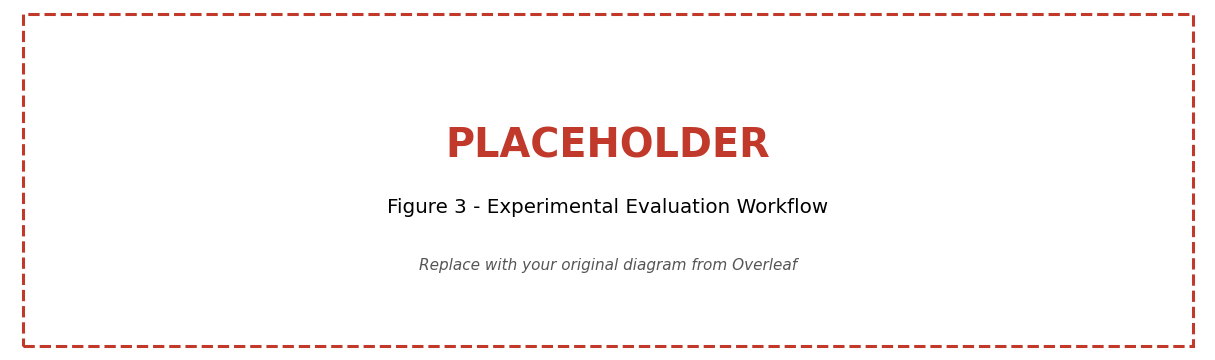
\includegraphics[width=\textwidth]{Figures/experimental_workflow.png}
    \caption{Experimental evaluation workflow.}
    \label{fig:experimental_workflow}
\end{figure*}

Con este propósito, se adoptó una estrategia de comparación controlada en la que las principales decisiones arquitectónicas se evaluaron en una infraestructura experimental común. Cada escenario experimental modifica únicamente una decisión de diseño, manteniendo constantes las demás condiciones de evaluación. Este enfoque proporciona un marco coherente para interpretar las diferencias observadas entre escenarios, minimizando la influencia de factores externos y facilitando el análisis del efecto individual de cada decisión arquitectónica sobre el comportamiento global del sistema.

\subsection{Experimental Design and Evaluation Strategy}
La evaluación experimental fue diseñada para analizar el comportamiento de la arquitectura propuesta como un sistema integrado para la detección de intrusiones en entornos IoT con recursos limitados. A diferencia de enfoques centrados en evaluar de manera independiente los componentes que conforman la solución, este trabajo busca determinar cómo las principales decisiones arquitectónicas influyen en el comportamiento global del sistema cuando la inferencia distribuida, el aprendizaje federado jerárquico y la protección de las comunicaciones operan de manera conjunta dentro de una infraestructura \textit{Edge--Fog--Cloud}. La Figura~\ref{fig:experimental_workflow} resume el flujo metodológico seguido para generar la evidencia experimental presentada en este trabajo.

Con el propósito de atribuir las diferencias observadas exclusivamente a las decisiones arquitectónicas objeto de estudio, todas las evaluaciones se realizaron según un protocolo experimental común. El conjunto de datos, la infraestructura de ejecución, el entorno de software, el protocolo de entrenamiento y las condiciones generales de evaluación permanecieron constantes durante toda la campaña experimental, mientras que únicamente se modificaron las variables independientes definidas para cada escenario. Este enfoque proporciona un marco metodológico coherente para analizar el efecto individual de cada decisión arquitectónica y reduce la influencia de factores externos sobre los resultados obtenidos.

La arquitectura incorpora un mecanismo de protección para las comunicaciones empleadas durante el proceso de aprendizaje federado, con el fin de preservar la confidencialidad, la autenticidad y la integridad de la información intercambiada entre los niveles \textit{Edge}, \textit{Fog} y \textit{Cloud}. En consecuencia, el diseño experimental considera un entorno operacional en el que la incorporación de dicho mecanismo constituye una decisión arquitectónica susceptible de influir en el desempeño global del sistema. Bajo esta perspectiva, la evaluación no pretende validar las propiedades criptográficas del algoritmo empleado, sino analizar el impacto de la protección de las comunicaciones sobre el comportamiento operacional de la arquitectura. En particular, se cuantifican los costos computacionales y de comunicación asociados a este mecanismo, lo que permite evaluar el equilibrio entre las garantías de seguridad proporcionadas y la eficiencia requerida para su despliegue en dispositivos IoT con recursos limitados.

En concordancia con los objetivos del estudio, las variables independientes fueron seleccionadas porque representan las tres decisiones arquitectónicas fundamentales introducidas por la propuesta: el modelo de inferencia ejecutado en los dispositivos \textit{Edge}, la organización del proceso de aprendizaje federado y el mecanismo de protección de las comunicaciones. Cada una de estas decisiones se evalúa mediante dos configuraciones alternativas, lo que permite construir un diseño factorial completo con ocho escenarios experimentales. La Tabla~\ref{tab:experimental_factors} resume los factores evaluados y las configuraciones consideradas.

\begin{table}[ht]
\centering
\caption{Variables independientes consideradas durante el diseño experimental.}
\label{tab:experimental_factors}
\footnotesize
\begin{tabular}{lcc}
\toprule
\textbf{Variable independiente} & \textbf{Configuración A} & \textbf{Configuración B} \\
\midrule
Modelo de inferencia & MLP & CNN \\
Arquitectura de aprendizaje federado & Edge--Cloud & Edge--Fog--Cloud \\
Protección de las comunicaciones & PLAIN & ASCON-128 \\
\bottomrule
\end{tabular}
\end{table}

La combinación sistemática de estas variables da lugar a un diseño factorial completo que permite cuantificar tanto el efecto individual de cada decisión arquitectónica como las posibles interacciones entre ellas, manteniendo constantes las demás condiciones experimentales. De este modo, la evidencia obtenida no se limita a comparar configuraciones particulares, sino que proporciona una base metodológica para analizar cómo las decisiones de diseño adoptadas inciden en el comportamiento global de la arquitectura propuesta.

Finalmente, la evaluación integra múltiples dimensiones de análisis con el propósito de caracterizar el comportamiento de la arquitectura desde una perspectiva funcional y operacional. Además del desempeño del sistema de detección de intrusiones, se evalúan el comportamiento del aprendizaje federado, la viabilidad de su despliegue en dispositivos con recursos limitados y el costo asociado a la incorporación del mecanismo de protección de las comunicaciones. Las siguientes subsecciones describen el conjunto de datos utilizado, el proceso de preparación de la información, la plataforma experimental, el protocolo de entrenamiento, los escenarios considerados y el marco metodológico empleado para responder a las preguntas de investigación planteadas en este trabajo.

\subsection{Conjunto de datos y preparación de la información}
Con el propósito de garantizar que todos los escenarios experimentales fueran evaluados bajo condiciones equivalentes, se definió un procedimiento uniforme para la construcción y preparación del conjunto de datos utilizado durante toda la campaña experimental. Este procedimiento comprende la adquisición del tráfico de red, su transformación en flujos unidireccionales (\textit{uniflows}), la extracción de características y el preprocesamiento de la información utilizada por los modelos de aprendizaje. La aplicación consistente de este proceso asegura que las diferencias observadas entre los escenarios experimentales sean consecuencia de las decisiones arquitectónicas evaluadas y no de variaciones en la preparación de los datos de entrada \cite{Hajj2023,Ficco2024}.

El conjunto de datos se construyó a partir de capturas de tráfico representativas de entornos IoT, seleccionadas por contener tanto comunicaciones legítimas como actividades maliciosas asociadas con el problema de detección de intrusiones abordado en este trabajo. En lugar de utilizar paquetes individuales, todas las comunicaciones se representaron mediante flujos unidireccionales, ya que este nivel de abstracción preserva el comportamiento estadístico del tráfico mientras reduce significativamente el volumen de información que debe procesarse durante la inferencia. Debido al equilibrio entre capacidad descriptiva y eficiencia computacional que ofrece este enfoque, las representaciones basadas en flujos se han consolidado como una de las alternativas más utilizadas para sistemas de detección de intrusiones basados en aprendizaje automático, particularmente en plataformas con recursos limitados \cite{Moustafa2019,CICIoT2023}.

Los flujos generados fueron organizados en tres clases de tráfico que representan el problema de clasificación considerado durante la evaluación experimental: tráfico legítimo, ataques de fuerza bruta contra el protocolo MQTT y actividades de exploración de red (\textit{network scanning}). En total, el conjunto de datos está compuesto por 256\,276 flujos unidireccionales. La Tabla~\ref{tab:dataset_composition} presenta la distribución de las clases empleadas en todos los experimentos.

\begin{table}[ht]
\centering
\caption{Clases de tráfico consideradas en la evaluación experimental.}
\label{tab:dataset_composition}
\footnotesize
\begin{tabular}{lrl}
\toprule
\textbf{Clase de tráfico} & \textbf{Flujos} & \textbf{Descripción} \\
\midrule
Normal & 171\,837 & Tráfico legítimo IoT \\
MQTT Brute Force & 33\,080 & Ataques de autenticación MQTT \\
Network Scan & 51\,359 & Actividades de reconocimiento de red \\
\midrule
\textbf{Total} & \textbf{256\,276} & Tres clases de tráfico \\
\bottomrule
\end{tabular}
\end{table}

Con el fin de mantener un equilibrio entre la capacidad discriminativa del modelo y las restricciones de memoria y de procesamiento impuestas por los dispositivos IoT, cada flujo se representó mediante un vector compacto de trece características estadísticas. Estas variables fueron seleccionadas para capturar cuatro dimensiones complementarias del comportamiento del tráfico de red: el volumen de comunicación, la dinámica temporal del flujo, la distribución del tamaño de los paquetes y el uso de banderas de control del protocolo TCP \cite{Zouhri2024,Li2017}. En conjunto, esta representación proporciona un nivel de abstracción suficiente para caracterizar el comportamiento de la comunicación y detectar actividades maliciosas, manteniendo al mismo tiempo un costo computacional compatible con las restricciones de memoria y de procesamiento propias de los dispositivos TinyML. La Tabla~\ref{tab:flow_features} resume las características utilizadas como entrada para todos los modelos evaluados.

\begin{table}[ht]
\centering
\caption{Características utilizadas para representar cada flujo de red como entrada de los modelos TinyML.}
\label{tab:flow_features}
\footnotesize
\begin{tabular}{lll}
\toprule
\textbf{Dimensión} & \textbf{Característica} & \textbf{Descripción} \\
\midrule
\multirow{2}{*}{Intensidad del flujo}
& \texttt{num\_pkts} & Número total de paquetes del flujo \\
& \texttt{num\_bytes} & Número total de bytes del flujo \\
\midrule

\multirow{4}{*}{Comportamiento temporal}
& \texttt{mean\_iat} & Tiempo promedio entre llegadas (IAT) \\
& \texttt{std\_iat} & Desviación estándar del IAT \\
& \texttt{min\_iat} & Valor mínimo del IAT \\
& \texttt{max\_iat} & Valor máximo del IAT \\
\midrule

\multirow{4}{*}{Longitud de paquetes}
& \texttt{mean\_pkt\_len} & Longitud promedio de los paquetes \\
& \texttt{std\_pkt\_len} & Desviación estándar de la longitud \\
& \texttt{min\_pkt\_len} & Longitud mínima de paquete \\
& \texttt{max\_pkt\_len} & Longitud máxima de paquete \\
\midrule

\multirow{3}{*}{Banderas TCP}
& \texttt{num\_psh\_flags} & Conteo de banderas PSH \\
& \texttt{num\_rst\_flags} & Conteo de banderas RST \\
& \texttt{num\_urg\_flags} & Conteo de banderas URG \\
\bottomrule
\end{tabular}
\end{table}

Antes del entrenamiento, todas las características fueron normalizadas mediante un procedimiento \textit{StandardScaler}, lo que transformó cada variable a media cero y varianza unitaria. Los parámetros de normalización obtenidos durante esta etapa fueron posteriormente incorporados al firmware de los dispositivos \textit{Edge}, lo que permitió aplicar exactamente la misma transformación durante la fase de inferencia. Esta estrategia garantiza la consistencia entre las fases de entrenamiento y despliegue, evitando discrepancias derivadas de diferencias en la escala de las variables de entrada y asegurando que todos los escenarios experimentales compartan una representación homogénea de la información utilizada por los modelos de aprendizaje.

\subsection{Plataforma experimental}
Todos los experimentos se realizaron en una plataforma experimental común, diseñada para implementar la arquitectura jerárquica \textit{Edge--Fog--Cloud} presentada en la Sección~\ref{sec:architecture}. Mantener un entorno de ejecución idéntico durante toda la campaña experimental garantiza que las diferencias observadas entre los escenarios evaluados sean consecuencia exclusiva de las decisiones arquitectónicas analizadas y no de variaciones en la infraestructura computacional subyacente. Esta configuración controlada proporciona una base reproducible para evaluar el impacto del aprendizaje federado jerárquico y de los mecanismos de criptografía ligera en sistemas distribuidos de detección de intrusiones para entornos IoT \cite{Wang2019,SaravanaBalaji2023}.

La plataforma experimental implementa la organización funcional propuesta para la arquitectura mediante tres niveles computacionales con responsabilidades claramente diferenciadas. Esta separación permite distribuir el ciclo completo de detección y aprendizaje entre dispositivos con capacidades heterogéneas, asignando cada proceso al nivel más adecuado desde el punto de vista computacional y reduciendo la carga sobre los dispositivos con recursos limitados.

La capa \textit{Edge} implementa las funciones de adquisición de tráfico e inferencia en tiempo real. En este nivel se capturan los flujos de red, se extraen las características utilizadas por el modelo de detección, se ejecuta la inferencia localmente mediante TinyML y se transmiten las actualizaciones necesarias para el proceso de aprendizaje distribuido. Asimismo, los dispositivos reciben periódicamente las nuevas versiones del modelo global, lo que permite mantener actualizada la capacidad de detección sin interrumpir la operación del sistema.

La capa \textit{Fog} implementa funciones de aprendizaje colaborativo cercanas a las fuentes de datos. Para ello, integra los componentes responsables de recibir la información proveniente de múltiples dispositivos \textit{Edge}, de mantener un buffer temporal de entrenamiento, de ejecutar el entrenamiento local y, cuando se emplea la arquitectura jerárquica, de realizar la agregación regional de los modelos antes de su envío al nivel superior. Esta organización reduce el volumen de información intercambiada con la nube y distribuye el proceso de aprendizaje a lo largo de la infraestructura.

La capa \textit{Cloud} implementa los servicios de coordinación global del sistema. Sus componentes funcionales realizan la agregación global mediante el algoritmo FedAvg, administran el repositorio del modelo global, coordinan las rondas sucesivas de aprendizaje federado y redistribuyen las nuevas versiones del modelo a la infraestructura distribuida. De esta forma, la coordinación global permanece desacoplada de las tareas de inferencia y entrenamiento locales, preservando la organización jerárquica característica de las arquitecturas \textit{Edge--Fog--Cloud} para aplicaciones IoT modernas \cite{Hajj2023,Ficco2024}.

La Figura~\ref{fig:architecture} resume la organización funcional de la plataforma experimental, mientras que las Tablas~\ref{tab:experimental_platform} y~\ref{tab:software_environment} presentan, respectivamente, la implementación de referencia utilizada durante la evaluación y el entorno de software empleado para materializar los componentes funcionales de cada nivel.

\begin{table}[ht]
\centering
\caption{Implementación de referencia de la plataforma experimental.}
\label{tab:experimental_platform}
\footnotesize
\begin{tabular}{l p{2.5cm}p{4cm}p{5cm}}
\toprule
\textbf{Nivel} &
\textbf{Implementación de referencia} &
\textbf{Componentes funcionales} &
\textbf{Responsabilidades} \\
\midrule

Edge & ESP32-S3 & Adquisición de tráfico, inferencia TinyML & Extracción de características, detección local de intrusiones, transmisión de información y recepción de actualizaciones del modelo global. \\

Fog & Raspberry Pi 4 Model B & Entrenamiento local, buffer de entrenamiento, agregación regional &
Recepción de información de dispositivos Edge, entrenamiento colaborativo, almacenamiento temporal de muestras y agregación regional del modelo (en modo jerárquico). \\

Cloud & Servidor Ubuntu & Agregación global, repositorio del modelo, orquestación &
Agregación mediante FedAvg, coordinación del aprendizaje federado, gestión del modelo global y redistribución de nuevas versiones del modelo. \\
\bottomrule
\end{tabular}
\end{table}

\begin{table}[ht]
\centering
\caption{Entorno de software utilizado en la plataforma experimental.}
\label{tab:software_environment}
\footnotesize
\begin{tabular}{l p{4.5cm}p{7cm}}
\toprule
\textbf{Nivel} &
\textbf{Tecnologías principales} &
\textbf{Propósito} \\
\midrule

Edge &
TensorFlow Lite for Microcontrollers &
Ejecución del modelo TinyML para la inferencia local y la extracción de características del tráfico. \\

Fog &
TensorFlow/Keras, Mosquitto MQTT Broker &
Entrenamiento local, almacenamiento temporal de muestras, comunicación con dispositivos Edge y agregación regional del modelo. \\

Cloud &
TensorFlow/Keras, FastAPI &
Agregación global mediante FedAvg, gestión del modelo global, coordinación de las rondas de aprendizaje y redistribución de modelos. \\

\bottomrule
\end{tabular}
\end{table}

La configuración de hardware, la infraestructura de comunicaciones y el entorno de software permanecieron invariables durante toda la campaña experimental. En consecuencia, todas las comparaciones se realizaron bajo condiciones de operación idénticas, modificando únicamente las variables experimentales definidas en la estrategia de evaluación. Esta decisión metodológica garantiza que las diferencias observadas puedan atribuirse directamente a las alternativas arquitectónicas propuestas y no a variaciones en la plataforma de ejecución, lo que fortalece la validez interna y la reproducibilidad de los resultados experimentales.

\subsection{Criterios de selección del modelo de inferencia para el despliegue en dispositivos \textit{Edge}}
La selección del modelo de inferencia constituye una decisión de diseño que condiciona el desarrollo de toda la evaluación experimental. A diferencia de los escenarios de entrenamiento centralizado, donde la capacidad de clasificación suele ser el principal criterio para comparar diferentes modelos de aprendizaje automático, el despliegue sobre dispositivos \textit{Edge} con recursos limitados introduce restricciones adicionales relacionadas con la memoria disponible, la capacidad de procesamiento, la latencia de inferencia y la compatibilidad con entornos TinyML. En consecuencia, la selección del modelo debe considerar simultáneamente los objetivos funcionales del sistema y la viabilidad de su implementación sobre la plataforma de despliegue.

La Figura~\ref{fig:model_selection_framework} resume los criterios de diseño considerados para seleccionar los modelos de inferencia incluidos en el diseño experimental. El proceso parte de dos conjuntos de requisitos complementarios. El primero corresponde a los objetivos funcionales del sistema de detección de intrusiones, que incluyen la capacidad de detección, la capacidad de generalización, la robustez del modelo y la eficiencia computacional requerida durante la inferencia. El segundo reúne las restricciones impuestas por la plataforma experimental, tales como la memoria disponible, la latencia de inferencia, la eficiencia energética y la compatibilidad con plataformas TinyML \cite{HeydariSurvey2025,Bartoli2025,Warden2019}. La integración de ambos conjuntos de criterios proporciona un marco de evaluación para analizar diferentes alternativas de aprendizaje automático, considerando simultáneamente su desempeño esperado y su factibilidad de despliegue en dispositivos \textit{Edge}.

\begin{figure*}[ht]
    \centering
    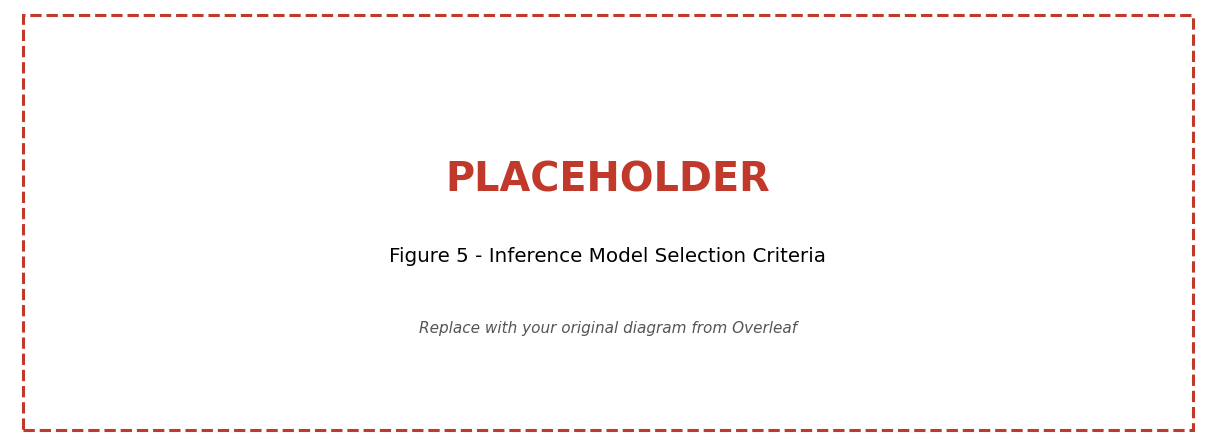
\includegraphics[width=\textwidth]{Figures/Model_Selection.png}
    \caption{Criterios funcionales y restricciones de despliegue considerados para la selección de los modelos de inferencia incluidos en el diseño experimental.}
    \label{fig:model_selection_framework}
\end{figure*}

Bajo estos criterios se analizaron diferentes modelos de aprendizaje automático representativos tanto de enfoques tradicionales como de arquitecturas compatibles con TinyML. Como resultado de este proceso, las arquitecturas MLP y CNN fueron seleccionadas como los niveles del factor experimental denominado \textit{Modelo de inferencia}, definido posteriormente en la Subsección~\ref{sec:experimental_scenarios}. La definición de estos niveles permite analizar el efecto que la complejidad del modelo puede ejercer sobre el comportamiento de la arquitectura propuesta bajo las condiciones experimentales establecidas. La validación experimental de esta decisión de diseño se presenta en la Sección~\ref{sec:results}.

\subsection{Protocolo experimental}
La evaluación experimental se realizó siguiendo un protocolo común de aprendizaje federado jerárquico para todos los escenarios considerados en este trabajo. Independientemente del modelo TinyML, de la arquitectura de aprendizaje o del mecanismo de protección de las comunicaciones evaluado, todas las configuraciones experimentales compartieron exactamente la misma secuencia de ejecución, lo que garantiza que las diferencias observadas en los resultados sean consecuencia exclusiva de las variables experimentales definidas en la estrategia de evaluación. La Figura~\ref{fig:experimental_protocol} resume las tres fases que componen cada ronda del protocolo experimental.

\begin{figure*}[ht]
    \centering
    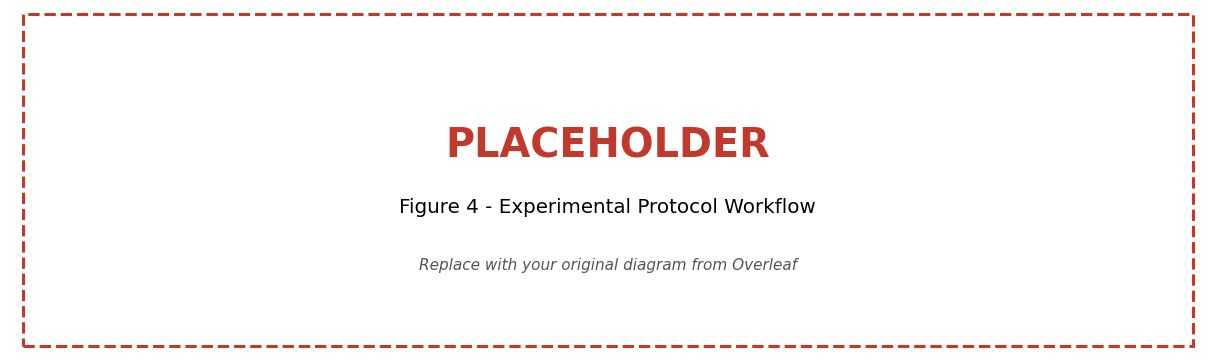
\includegraphics[width=\textwidth]{Figures/experimental_protocol.png}
    \caption{Experimental protocol workflow.}
    \label{fig:experimental_protocol}
\end{figure*}

Cada ronda del aprendizaje federado se estructura en tres fases consecutivas: sincronización del modelo global, aprendizaje local y agregación federada.

\textbf{Fase 1. Sincronización del modelo global.}
Al inicio de cada ronda, la capa \textit{Cloud} distribuye la versión más reciente del modelo global a los nodos \textit{Fog}, que posteriormente la sincronizan con los dispositivos \textit{Edge}. Este procedimiento garantiza que todos los participantes inicien el proceso de entrenamiento a partir de un modelo consistente, evitando divergencias derivadas del uso de versiones distintas en la misma ronda de aprendizaje \cite{McMahan2017,Imteaj2022}.

\textbf{Fase 2. Inferencia y aprendizaje local.}
Una vez sincronizado el modelo, los dispositivos \textit{Edge} ejecutan de forma continua el proceso de inferencia sobre el tráfico observado en sus respectivos dominios de operación. Las características extraídas se envían al nodo \textit{Fog}, donde se almacenan temporalmente en un buffer de entrenamiento de tamaño fijo ($N_s=40$ muestras). Cuando el buffer alcanza su capacidad, las muestras se etiquetan mediante un mecanismo heurístico basado en el resultado del proceso de detección y se incorporan al conjunto local de entrenamiento.

El entrenamiento local se ejecuta durante cinco épocas, con un tamaño de lote (\textit{batch size}) de 8 muestras. Con el propósito de reducir el volumen de comunicación y preservar la naturaleza distribuida del aprendizaje federado, únicamente se comparten los parámetros de las capas finales de clasificación del modelo, mientras que las capas encargadas de la extracción de representaciones permanecen inalteradas en cada nodo local.

\textbf{Fase 3. Agregación federada y actualización del modelo.}
Finalizado el entrenamiento local, cada nodo \textit{Fog} transmite únicamente la actualización de los parámetros del modelo, sin compartir las muestras empleadas durante el entrenamiento. En la arquitectura jerárquica, los gateways realizan primero una agregación regional antes de remitir los modelos consolidados al coordinador global. Posteriormente, la capa \textit{Cloud} aplica el algoritmo FedAvg para construir una nueva versión del modelo global, la almacena en el repositorio central y la redistribuye a toda la infraestructura para iniciar la siguiente ronda de aprendizaje. Este procedimiento mantiene sincronizados a todos los participantes, preserva la privacidad de los datos utilizados durante el entrenamiento y reduce el volumen de información intercambiada entre los distintos niveles de la arquitectura \cite{McMahan2017,Ramadan2025}.

La Tabla~\ref{tab:federated_parameters} resume la configuración adoptada para la ejecución del protocolo de aprendizaje federado y la justificación metodológica de cada parámetro utilizado.

\begin{table}[ht]
\centering
\caption{Configuración del protocolo de aprendizaje federado.}
\label{tab:federated_parameters}
\footnotesize
\begin{tabular}{p{3.3cm}p{2.8cm}p{6.4cm}}
\toprule
\textbf{Parámetro} & \textbf{Configuración} & \textbf{Justificación} \\
\midrule

Buffer de entrenamiento & 40 muestras & Proporciona un conjunto representativo para el entrenamiento local, manteniendo una frecuencia adecuada de actualización del modelo. \\

Épocas de entrenamiento local & 5 & Permite alcanzar la convergencia local limitando el costo computacional en los nodos \textit{Fog}. \\

Tamaño de lote (\textit{batch size}) & 8 & Equilibra la estabilidad del proceso de optimización y el consumo de memoria durante el entrenamiento local. \\

Algoritmo de agregación & FedAvg & Realiza una agregación ponderada de los modelos locales para construir el modelo global compartido. \\

Información compartida & Parámetros de las capas finales del modelo & Reduce el volumen de comunicación preservando las representaciones aprendidas localmente y manteniendo la naturaleza distribuida del entrenamiento. \\

Datos compartidos & Ninguno & Garantiza que las muestras de entrenamiento permanezcan en el dominio en el que fueron generadas, preservando la privacidad de la información. \\

Sincronización del modelo & Inicio de cada ronda & Asegura que todos los participantes comiencen el entrenamiento a partir de una versión consistente del modelo global. \\

Actualización del modelo global & Final de cada ronda & Incorpora el conocimiento adquirido por todos los participantes antes de iniciar la siguiente iteración del aprendizaje federado. \\

\bottomrule
\end{tabular}
\end{table}

Durante toda la campaña experimental permanecieron constantes el conjunto de datos, la infraestructura de hardware, el entorno de software, la configuración del protocolo de aprendizaje federado y los hiperparámetros de entrenamiento. En contraste, las únicas variables modificadas entre escenarios correspondieron al modelo TinyML utilizado, a la arquitectura de aprendizaje federado y al mecanismo de protección de las comunicaciones. Esta separación entre condiciones controladas y variables experimentales garantiza la comparabilidad entre todas las configuraciones evaluadas y constituye la base metodológica para el análisis de los escenarios experimentales presentado en la siguiente subsección.

\subsection{Escenarios experimentales}
\label{sec:experimental_scenarios}
La evaluación experimental se realizó mediante un diseño factorial completo con el propósito de analizar, de forma sistemática y reproducible, el efecto individual y combinado de las principales decisiones arquitectónicas propuestas en este trabajo. Todas las configuraciones experimentales se ejecutaron utilizando la misma plataforma y el mismo protocolo descritos en las subsecciones anteriores, garantizando que las diferencias observadas durante la evaluación fueran consecuencia exclusiva de las variables arquitectónicas bajo estudio.

Las configuraciones experimentales fueron generadas mediante la combinación de tres factores arquitectónicos independientes que representan las principales decisiones de diseño de la solución propuesta: la arquitectura del aprendizaje federado, el modelo TinyML desplegado en los dispositivos \textit{Edge} y el mecanismo de protección de las comunicaciones empleado durante el intercambio de los parámetros del modelo.

El primer factor corresponde a la arquitectura del aprendizaje federado y compara una organización convencional \textit{Edge--Cloud}, en la cual todos los modelos locales se envían directamente al coordinador global, con la arquitectura jerárquica \textit{Edge--Fog--Cloud} propuesta en este trabajo, en la que la capa \textit{Fog} incorpora una etapa intermedia de entrenamiento local y agregación regional antes de la sincronización global.

El segundo factor evalúa el modelo TinyML utilizado para la detección de intrusiones en los dispositivos \textit{Edge}. Para ello, se consideran dos arquitecturas representativas con diferentes complejidades computacionales: un perceptrón multicapa (\textit{MLP}) y una red neuronal convolucional unidimensional (\textit{CNN-1D}). Esta comparación permite analizar el compromiso entre la capacidad de detección y el costo computacional en dispositivos IoT con recursos limitados.

Finalmente, el tercer factor estudia el efecto de incorporar mecanismos de criptografía ligera durante el proceso de aprendizaje federado. Para este propósito, se compara una configuración en la que las actualizaciones del modelo se intercambian sin protección criptográfica (\textit{Plaintext}) con una configuración equivalente protegida mediante ASCON-128, lo que permite cuantificar el impacto del mecanismo criptográfico en el intercambio de los parámetros del modelo.

La combinación de estos tres factores binarios genera un diseño factorial completo con $2^{3}=8$ configuraciones experimentales. Cada configuración representa una combinación única de las decisiones arquitectónicas consideradas en este trabajo. En consecuencia, el diseño experimental permite analizar tanto el efecto individual de cada factor como las posibles interacciones entre ellos en condiciones experimentales idénticas.

La Tabla~\ref{tab:experimental_design} resume los factores arquitectónicos considerados en la evaluación, así como las ocho configuraciones experimentales derivadas del diseño factorial. Estas configuraciones constituyen las unidades experimentales empleadas en el análisis comparativo presentado en la Sección de Resultados.

\begin{table*}[ht]
\centering
\caption{Diseño factorial utilizado para evaluar la arquitectura propuesta.}
\label{tab:experimental_design}
\footnotesize

\textbf{(A) Factores arquitectónicos}

\vspace{0.2cm}

\begin{tabular}{p{2.75cm}p{2.5cm}p{2.75cm}p{4cm}}
\toprule
\textbf{Factor arquitectónico} &
\textbf{Nivel 1} &
\textbf{Nivel 2} &
\textbf{Objetivo de evaluación} \\
\midrule

Arquitectura de aprendizaje federado &
Plana (\textit{Edge--Cloud}) &
Jerárquica (\textit{Edge--Fog--Cloud}) &
Evaluar la contribución de la agregación jerárquica al proceso de aprendizaje federado. \\

Modelo de inferencia TinyML &
MLP &
CNN-1D &
Analizar el impacto de la complejidad del modelo en el desempeño de la detección y en el costo computacional en la capa \textit{Edge}. \\

Protección de las comunicaciones &
Plaintext &
ASCON-128 &
Cuantificar el impacto de la criptografía ligera durante el intercambio de los parámetros del modelo federado. \\

\bottomrule
\end{tabular}

\vspace{0.5cm}

\textbf{(B) Configuraciones experimentales}

\vspace{0.2cm}

\begin{tabular}{cccc}
\toprule
\textbf{Escenario} &
\textbf{Arquitectura FL} &
\textbf{Modelo TinyML} &
\textbf{Protección} \\
\midrule

E1 & Plana & MLP & ASCON-128 \\
E2 & Plana & MLP & Plaintext \\
E3 & Jerárquica & MLP & ASCON-128 \\
E4 & Jerárquica & MLP & Plaintext \\
E5 & Plana & CNN-1D & ASCON-128 \\
E6 & Plana & CNN-1D & Plaintext \\
E7 & Jerárquica & CNN-1D & ASCON-128 \\
E8 & Jerárquica & CNN-1D & Plaintext \\

\bottomrule
\end{tabular}

\end{table*}

\subsection{Estrategia de evaluación}
El diseño factorial presentado en la subsección anterior define las configuraciones experimentales empleadas para evaluar la arquitectura propuesta. Sin embargo, el propósito del estudio no consiste únicamente en comparar dichas configuraciones, sino en analizar el efecto de las principales decisiones arquitectónicas en diferentes dimensiones del comportamiento del sistema. Para ello, la evidencia experimental se organizó en torno a un conjunto de preguntas de investigación que permiten analizar de manera sistemática la contribución de cada factor considerado en el diseño experimental.

Las preguntas de investigación constituyen el eje organizador del análisis experimental y establecen una relación explícita entre el diseño experimental, las comparaciones realizadas y la organización de los resultados. Esta estrategia permite estudiar de forma independiente el desempeño global del sistema, el efecto de la arquitectura de aprendizaje federado, el impacto del modelo TinyML y la incorporación de mecanismos de criptografía ligera, evitando comparaciones redundantes y facilitando la interpretación de los resultados.

La Tabla~\ref{tab:evaluation_strategy} resume la estrategia de evaluación empleada en este trabajo. Para cada pregunta de investigación se identifican el objetivo del análisis, el factor arquitectónico asociado y las comparaciones experimentales requeridas para responderla. De esta manera, se establece una trazabilidad explícita entre el diseño experimental presentado en la subsección anterior y la organización de los resultados desarrollada en la Sección~\ref{sec:results}.

\begin{table*}[ht]
\centering
\caption{Estrategia de evaluación utilizada en el análisis experimental.}
\label{tab:evaluation_strategy}
\footnotesize

\begin{tabularx}{\textwidth}{l p{3.5cm} p{3.5cm} X}
\toprule
\textbf{RQ} &
\textbf{Objetivo del análisis} &
\textbf{Factor arquitectónico} &
\textbf{Comparaciones experimentales} \\
\midrule

\textbf{RQ1} &
Evaluar el desempeño global del sistema de detección de intrusiones propuesto. &
Desempeño global del sistema &
Análisis comparativo de todas las configuraciones experimentales para caracterizar el comportamiento general del IDS bajo las distintas combinaciones de los factores arquitectónicos. \\

\textbf{RQ2} &
Analizar el efecto de la arquitectura jerárquica de aprendizaje federado en el desempeño del sistema. &
Arquitectura de aprendizaje federado &
Comparación entre las arquitecturas convencionales (\textit{Edge--Cloud}) y jerárquicas (\textit{Edge--Fog--Cloud}) para evaluar la contribución de la agregación regional incorporada por la capa \textit{Fog}. \\

\textbf{RQ3} &
Evaluar el impacto del modelo TinyML en el desempeño y el costo computacional del sistema. &
Modelo de inferencia TinyML &
Comparación entre los modelos MLP y CNN-1D para analizar el compromiso entre la capacidad de detección y los requisitos computacionales en dispositivos \textit{Edge}. \\

\textbf{RQ4} &
Cuantificar el impacto de la criptografía ligera en el proceso de aprendizaje federado. &
Protección de las comunicaciones &
Comparación entre las configuraciones \textit{Plaintext} y ASCON-128 para determinar el costo asociado a proteger el intercambio de los parámetros del modelo. \\

\bottomrule
\end{tabularx}

\end{table*}

Aunque el diseño experimental contempla ocho configuraciones distintas, cada pregunta de investigación utiliza únicamente las comparaciones necesarias para aislar el efecto del factor arquitectónico bajo estudio, manteniendo constantes las demás variables siempre que sea posible. Este enfoque facilita la interpretación de los resultados y permite atribuir las diferencias observadas a las decisiones de diseño evaluadas.

Finalmente, la siguiente subsección presenta las métricas empleadas para responder cada una de las preguntas de investigación, describiendo su definición formal, el procedimiento utilizado para su cálculo y los criterios considerados para interpretar los resultados experimentales.

\subsection{Métricas de evaluación}
\label{sec:evaluation_metrics}
La evaluación de la arquitectura propuesta requiere un conjunto de métricas que permitan caracterizar las distintas dimensiones funcionales y operacionales del sistema. Debido a que la solución integra mecanismos de detección de intrusiones, aprendizaje federado jerárquico, computación \textit{Edge} y comunicaciones seguras mediante criptografía ligera, ninguna métrica individual es suficiente para describir de manera integral su comportamiento. En consecuencia, se definió un conjunto de indicadores complementarios que permiten evaluar cada una de las dimensiones consideradas en el estudio.

Las métricas empleadas se organizaron en cuatro categorías de evaluación: desempeño del sistema de detección de intrusiones, desempeño del aprendizaje federado, desempeño del despliegue en dispositivos \textit{Edge} y desempeño de las comunicaciones seguras. Cada categoría reúne los indicadores necesarios para caracterizar una dimensión específica de la arquitectura y proporciona la evidencia cuantitativa empleada en el análisis experimental.

La Tabla~\ref{tab:metrics_mapping} resume las categorías de evaluación consideradas, las preguntas de investigación a las que contribuyen y las principales métricas utilizadas en los experimentos.

\begin{table}[ht]
\centering
\caption{Relación entre las categorías de evaluación, las preguntas de investigación y las métricas empleadas en la evaluación experimental.}
\label{tab:metrics_mapping}
\footnotesize

\begin{tabularx}{\columnwidth}{p{3.5cm} c X}
\toprule
\textbf{Categoría de evaluación} & \textbf{RQ} & \textbf{Métricas principales} \\
\midrule

Desempeño del sistema de detección de intrusiones &  RQ1 & Accuracy, Precision, Recall y F1-score. \\

Desempeño del aprendizaje federado & RQ2 & Exactitud global del modelo, pérdida de entrenamiento y velocidad de convergencia. \\

Desempeño del despliegue en dispositivos \textit{Edge} & RQ3 & Latencia de inferencia y huella de memoria del modelo desplegado. \\

Desempeño de las comunicaciones seguras & RQ4 & Tiempo de cifrado, tiempo de descifrado y sobrecarga de comunicación. \\

\bottomrule
\end{tabularx}
\end{table}

Las siguientes subsecciones describen las métricas de cada categoría de evaluación. Las métricas ampliamente consolidadas en la literatura se presentan de forma concisa junto con su formulación matemática cuando resulta pertinente. En contraste, las métricas específicas del aprendizaje federado y del comportamiento de la infraestructura distribuida se describen, enfatizando el procedimiento de medición empleado en los experimentos y los criterios adoptados para interpretar los resultados.

\subsubsection{Desempeño del sistema de detección de intrusiones}
El desempeño del sistema de detección de intrusiones se evaluó mediante un conjunto de métricas de clasificación ampliamente utilizadas en modelos de aprendizaje supervisado. Todas las métricas se calcularon a partir de la matriz de confusión obtenida en cada configuración experimental, considerando el número de verdaderos positivos ($TP$), verdaderos negativos ($TN$), falsos positivos ($FP$) y falsos negativos ($FN$).

Las métricas empleadas corresponden a la exactitud (\textit{Accuracy}), la precisión (\textit{Precision}), la sensibilidad (\textit{Recall}) y la medida F1 (\textit{F1-score}), cuyas definiciones matemáticas se presentan en las Ecuaciones~(\ref{eq:accuracy})--(\ref{eq:f1}).

\begin{align}
Accuracy &= \frac{TP+TN}{TP+TN+FP+FN}
\label{eq:accuracy}\\[2mm]
Precision &= \frac{TP}{TP+FP}
\label{eq:precision}\\[2mm]
Recall &= \frac{TP}{TP+FN}
\label{eq:recall}\\[2mm]
F1 &= 2\cdot\frac{Precision \times Recall}{Precision+Recall}
\label{eq:f1}
\end{align}

Estas métricas proporcionan una caracterización complementaria del desempeño del IDS. La exactitud ofrece una medida global de la capacidad de clasificación del sistema; la precisión evalúa la confiabilidad de las alertas generadas al cuantificar el efecto de los falsos positivos; la sensibilidad mide la capacidad del modelo para identificar correctamente los eventos maliciosos; y la medida F1 integra precisión y sensibilidad en un único indicador, proporcionando una evaluación robusta cuando existe desbalance entre las clases.

En conjunto, estos indicadores permiten evaluar de manera integral la capacidad de detección del sistema y comparar su desempeño en las diferentes configuraciones experimentales consideradas en este trabajo.

\subsubsection{Desempeño del aprendizaje federado}
El desempeño del proceso de aprendizaje federado se evaluó con el propósito de determinar si la arquitectura jerárquica propuesta permite construir un modelo global estable, eficiente y con capacidad de generalización. A diferencia de las métricas de clasificación utilizadas para evaluar el sistema de detección de intrusiones, esta categoría analiza el comportamiento del proceso de entrenamiento distribuido y la evolución del modelo global a lo largo de las rondas sucesivas de aprendizaje federado.

Como se ilustra en la Figura~\ref{fig:fl_evaluation_framework}, la evaluación del aprendizaje federado se estructuró en torno a tres dimensiones complementarias. La primera, \textit{Model Quality}, evalúa la calidad del modelo global mediante la evolución de la exactitud global (\textit{Global Accuracy}) a lo largo del entrenamiento. La segunda, \textit{Training Dynamics}, caracteriza la estabilidad del proceso de optimización mediante la evolución de la función de pérdida (\textit{Training Loss}) como indicador de convergencia y de consistencia del entrenamiento distribuido. Finalmente, la dimensión \textit{Learning Efficiency} cuantifica la eficiencia del proceso de aprendizaje mediante la velocidad de convergencia (\textit{Convergence Speed}), lo que permite comparar la rapidez con la que las distintas configuraciones experimentales alcanzan un modelo global estable \cite{Cooray2025,Ma2024}.

\begin{figure}[ht]
\centering
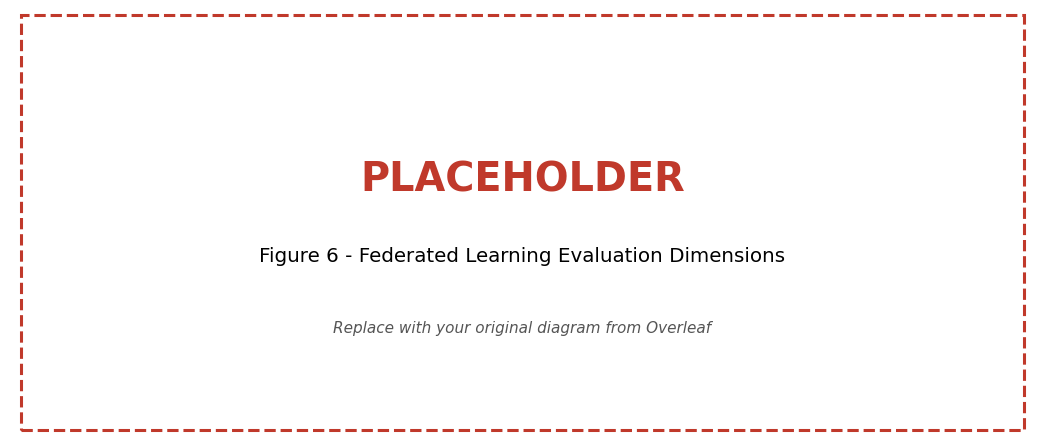
\includegraphics[width=\linewidth]{Figures/fl_evaluation_framework.png}
\caption{Dimensiones consideradas para evaluar el desempeño del aprendizaje federado.}
\label{fig:fl_evaluation_framework}
\end{figure}

En conjunto, estas tres dimensiones proporcionan una caracterización integral del proceso de aprendizaje federado al evaluar la calidad del modelo global, la estabilidad del entrenamiento distribuido y la eficiencia con la que el conocimiento generado localmente se incorpora al modelo compartido. La combinación de estos indicadores permite analizar el efecto de la arquitectura jerárquica sobre el comportamiento del aprendizaje federado y comparar las diferentes configuraciones experimentales consideradas en este trabajo.

\subsubsection{Desempeño del despliegue en dispositivos \textit{Edge}}
La tercera dimensión de evaluación se orientó a analizar el desempeño del sistema de detección de intrusiones durante su ejecución en dispositivos \textit{Edge}. Mientras que las subsecciones anteriores evaluaron la capacidad de detección del modelo y el comportamiento del proceso de aprendizaje federado, esta etapa se centra en determinar la viabilidad de desplegar el modelo entrenado en plataformas con recursos computacionales limitados, garantizando tiempos de respuesta adecuados y un uso eficiente de los recursos disponibles.

La evaluación se centra en el proceso de inferencia ejecutado localmente en los nodos \textit{Edge}, donde el modelo global, obtenido mediante aprendizaje federado, procesa el tráfico de red para identificar actividades maliciosas sin depender de un procesamiento continuo en la nube. En este contexto, el interés no radica únicamente en la capacidad de detección del modelo, sino también en el costo computacional asociado a su ejecución en plataformas con restricciones de procesamiento y memoria propias de los dispositivos IoT.

Para caracterizar este comportamiento se definieron dos dimensiones complementarias de evaluación. La primera, \textit{Execution Performance}, analiza la capacidad de respuesta del sistema mediante la latencia de inferencia (\textit{Inference Latency}), lo que permite determinar si el modelo satisface los requisitos temporales de las aplicaciones IoT con restricciones de tiempo de respuesta. La segunda, \textit{Resource Utilization}, evalúa la demanda de memoria impuesta por el modelo desplegado mediante su huella de memoria (\textit{Model Footprint}), como indicador del impacto de la ejecución sobre los recursos disponibles del dispositivo \cite{HeydariSurvey2025,Bartoli2025}.

En conjunto, estas dos dimensiones proporcionan una caracterización integral del desempeño del sistema durante su ejecución en plataformas \textit{Edge}. La combinación de la capacidad de respuesta y el uso eficiente de los recursos computacionales permite evaluar la viabilidad del despliegue del sistema de detección de intrusiones en dispositivos IoT con recursos limitados.

\subsubsection{Desempeño de las comunicaciones seguras}
La cuarta dimensión de evaluación se orientó a analizar el desempeño del mecanismo de comunicación segura incorporado para proteger el intercambio de información entre los componentes de la arquitectura Cloud--Fog--Edge. Mientras que las subsecciones anteriores evaluaron el desempeño funcional del sistema de detección de intrusiones, el proceso de aprendizaje federado y el despliegue del modelo en dispositivos \textit{Edge}, esta etapa se centra en cuantificar el impacto computacional asociado a la incorporación de un mecanismo criptográfico basado en ASCON, garantizando la confidencialidad e integridad de la información sin comprometer la eficiencia operativa de la arquitectura.

La evaluación se centra en las operaciones criptográficas realizadas durante el intercambio de modelos, parámetros y mensajes de control entre las capas \textit{Cloud}, \textit{Fog} y \textit{Edge}. En este contexto, el interés no radica únicamente en verificar la protección de las comunicaciones, sino también en determinar el costo computacional asociado a su incorporación en plataformas con las restricciones de procesamiento y memoria propias de los entornos IoT.

Para caracterizar este comportamiento se definieron dos dimensiones complementarias de evaluación. La primera, \textit{Cryptographic Performance}, analiza el desempeño temporal del mecanismo de protección mediante el tiempo de cifrado (\textit{Encryption Time}) y el de descifrado (\textit{Decryption Time}), lo que permite cuantificar el retardo introducido por las operaciones criptográficas. La segunda, \textit{Communication Overhead}, evalúa el incremento del volumen de información transmitida como consecuencia del encapsulamiento autenticado de los parámetros intercambiados \cite{Sorescu2025,Alshammari2026}.

En conjunto, estas dos dimensiones proporcionan una caracterización integral del desempeño de las comunicaciones seguras al evaluar tanto el costo temporal de las operaciones criptográficas como el incremento del tráfico asociado. La combinación de estos indicadores permite determinar la viabilidad de incorporar mecanismos de comunicación segura en arquitecturas IoT distribuidas preservando un desempeño compatible con sus restricciones operacionales.

%%%%%%%%%%%%%%%%%%%%%%%%%%%%%%%%%%%%%%%%%%
\section{Resultados}
\label{sec:results}
Esta sección presenta la validación de la arquitectura de detección de intrusiones \textit{Edge--Fog--Cloud} propuesta. En lugar de evaluar de manera independiente los componentes que la conforman, el análisis se centra en validar las principales decisiones de diseño incorporadas durante el desarrollo de la arquitectura y determinar cómo su integración influye sobre el comportamiento global del sistema bajo condiciones representativas de despliegue. De esta manera, la evidencia se organiza alrededor de las decisiones arquitectónicas que sustentan la solución propuesta, permitiendo analizar de forma sistemática la contribución de cada una de ellas al desempeño funcional y operacional del sistema.

La evaluación se desarrolla de manera progresiva, siguiendo una secuencia en la que cada propiedad analizada constituye el fundamento para interpretar la siguiente. Inicialmente, se verifica la viabilidad de ejecutar el proceso de inferencia sobre dispositivos \textit{Edge} con recursos limitados, validando la decisión de seleccionar modelos compatibles con TinyML para satisfacer las restricciones de despliegue impuestas por la plataforma experimental. Posteriormente, se analiza el comportamiento del proceso de aprendizaje federado jerárquico mediante el estudio de su convergencia, estabilidad y desempeño colaborativo. Una vez establecidas estas propiedades, se evalúa la capacidad de detección de la arquitectura integrada para determinar si las decisiones de diseño preservan la funcionalidad principal del sistema como mecanismo de detección de intrusiones. Finalmente, se analiza el costo operacional asociado al aprendizaje federado jerárquico y el impacto de incorporar comunicaciones seguras mediante ASCON-128 durante el intercambio de parámetros del modelo federado. En conjunto, estos resultados proporcionan una validación integral de la arquitectura propuesta bajo las condiciones definidas en la metodología.

\subsection{Validación del modelo de inferencia para el despliegue en dispositivos \textit{Edge}}
La metodología estableció que las restricciones propias del despliegue sobre dispositivos \textit{Edge} condicionan la selección del modelo de inferencia y justifican la incorporación de arquitecturas compatibles con TinyML. En esta subsección se valida experimentalmente dicha decisión mediante una comparación entre modelos tradicionales de aprendizaje automático y modelos diseñados para su ejecución sobre plataformas con recursos limitados.

La Tabla~\ref{tab:model_comparison} resume los resultados obtenidos durante esta evaluación. Además de la capacidad de detección, la comparación incorpora indicadores de huella de memoria y tiempo de inferencia medidos sobre la plataforma ESP32-S3, permitiendo analizar simultáneamente el desempeño predictivo y la viabilidad de despliegue de cada alternativa.

\begin{table*}[htb]
\caption{Comparison of inference models considering detection performance and Edge deployment constraints.}
\label{tab:model_comparison}
\centering
\footnotesize
\begin{tabular}{lccc}
\toprule

&
\textbf{Detection} & \multicolumn{2}{c}{\textbf{Edge Deployment Constraints}} \\
\cmidrule(lr){2-2}
\cmidrule(lr){3-4}

\textbf{Candidate Model} & \textbf{Accuracy (\%)} & \textbf{Model Footprint} & \textbf{Inference Time (ms)} \\

\midrule
\addlinespace
\multicolumn{4}{l}{\textit{Classical Machine Learning Models}} \\
\addlinespace

Decision Tree   &   99.87           &   $\sim$15 KB     &   $<$0.1 \\
Random Forest   &   \textbf{99.94}  &   $\sim$2.5 MB    &   $\sim$5 \\
SVM (RBF)       &   99.68           &   $\sim$4 MB      &   $\sim$50 \\

\addlinespace
\multicolumn{4}{l}{\textit{TinyML Models}} \\
\addlinespace

CNN-1D  &   90.51   &   $\sim$18 KB             &   $<$0.5  \\
MLP     &   90.60   &   \textbf{$\sim$4.5 KB}   &   \textbf{$<$0.1} \\

\bottomrule
\end{tabular}
\vspace{2mm}
\begin{flushleft}
\footnotesize\textit{Note:} Model footprint and inference time correspond to the implementation on the target ESP32-S3 Edge platform.
\end{flushleft}
\end{table*}

Si el análisis se limitara exclusivamente a la capacidad de clasificación, los modelos tradicionales constituirían la mejor alternativa. Random Forest alcanza el mayor nivel de precisión, seguido por Decision Tree y SVM, superando el desempeño obtenido por las arquitecturas compatibles con TinyML.

Sin embargo, esta conclusión cambia al incorporar las restricciones propias del despliegue sobre dispositivos \textit{Edge}. Aunque los modelos tradicionales ofrecen un mejor desempeño predictivo, sus requerimientos de memoria y sus tiempos de inferencia exceden las capacidades disponibles en la plataforma ESP32-S3, limitando su utilización en el escenario de despliegue considerado. En consecuencia, la selección del modelo deja de depender exclusivamente de la precisión alcanzada y pasa a considerar simultáneamente la capacidad de detección y la viabilidad de implementación sobre el hardware objetivo.

Bajo estas condiciones, las arquitecturas compatibles con TinyML representan la única alternativa capaz de satisfacer simultáneamente los requisitos funcionales del sistema y las restricciones computacionales de la plataforma de despliegue. Tanto MLP como CNN presentan capacidades de detección similares, manteniendo huellas de memoria y tiempos de inferencia compatibles con la ejecución sobre el dispositivo \textit{Edge}. Estos resultados confirman que la reducción de complejidad inherente a las arquitecturas TinyML permite preservar una capacidad de detección adecuada sin comprometer la viabilidad del despliegue.

Entre los modelos TinyML evaluados, la arquitectura MLP presenta la menor huella de memoria y el menor tiempo de inferencia, manteniendo un desempeño de clasificación comparable al obtenido por la CNN. Por esta razón, la MLP fue seleccionada como modelo principal para el proceso de inferencia, mientras que la CNN se conservó como arquitectura de referencia para analizar la influencia del modelo de inferencia sobre el comportamiento global del sistema distribuido durante las evaluaciones posteriores.

En conjunto, la evidencia experimental valida la decisión metodológica de seleccionar modelos compatibles con TinyML para el despliegue sobre dispositivos \textit{Edge}. Los resultados demuestran que, bajo restricciones computacionales representativas de plataformas IoT, la selección del modelo de inferencia constituye una decisión arquitectónica en la que la capacidad de detección debe evaluarse conjuntamente con la eficiencia computacional y la viabilidad de implementación. Esta validación establece la base para las siguientes evaluaciones, donde se analiza si el modelo seleccionado mantiene un proceso de aprendizaje colaborativo estable dentro de la arquitectura federada propuesta.

\subsection{Validación del proceso de aprendizaje colaborativo}
La subsección anterior validó la selección del modelo de inferencia para su despliegue sobre dispositivos \textit{Edge}. Una vez establecida la viabilidad de esta decisión de diseño, el siguiente paso consiste en verificar que dicho modelo puede entrenarse de manera colaborativa dentro de la arquitectura \textit{Edge--Fog--Cloud}. La incorporación de múltiples niveles de agregación, la coordinación entre nodos distribuidos y la protección de las comunicaciones durante el intercambio de parámetros pueden influir sobre la dinámica del aprendizaje federado. En consecuencia, antes de evaluar la capacidad de detección de la arquitectura, resulta necesario demostrar que el proceso de aprendizaje converge de manera consistente y mantiene una dinámica de optimización estable bajo las diferentes configuraciones experimentales consideradas.

La primera propiedad evaluada corresponde a la convergencia del proceso de aprendizaje federado. La Figura~\ref{fig:convergence} muestra la evolución del \textit{accuracy} global y de la función de pérdida durante las primeras veinte rondas de entrenamiento para los ocho escenarios experimentales definidos en la metodología. A pesar de las diferencias propias de cada configuración, todas las variantes presentan una evolución similar, caracterizada por un incremento progresivo del \textit{accuracy} acompañado por una reducción sostenida de la pérdida. Durante las primeras rondas se observa una rápida mejora del modelo global, seguida por una etapa de estabilización en la que las ganancias adicionales de desempeño disminuyen gradualmente hasta alcanzar un régimen de operación estable. En conjunto, estos resultados demuestran que la estrategia de aprendizaje federado jerárquico implementada permite optimizar el modelo global de manera consistente, independientemente de la configuración arquitectónica evaluada.

\begin{figure*}[ht]
    \centering
    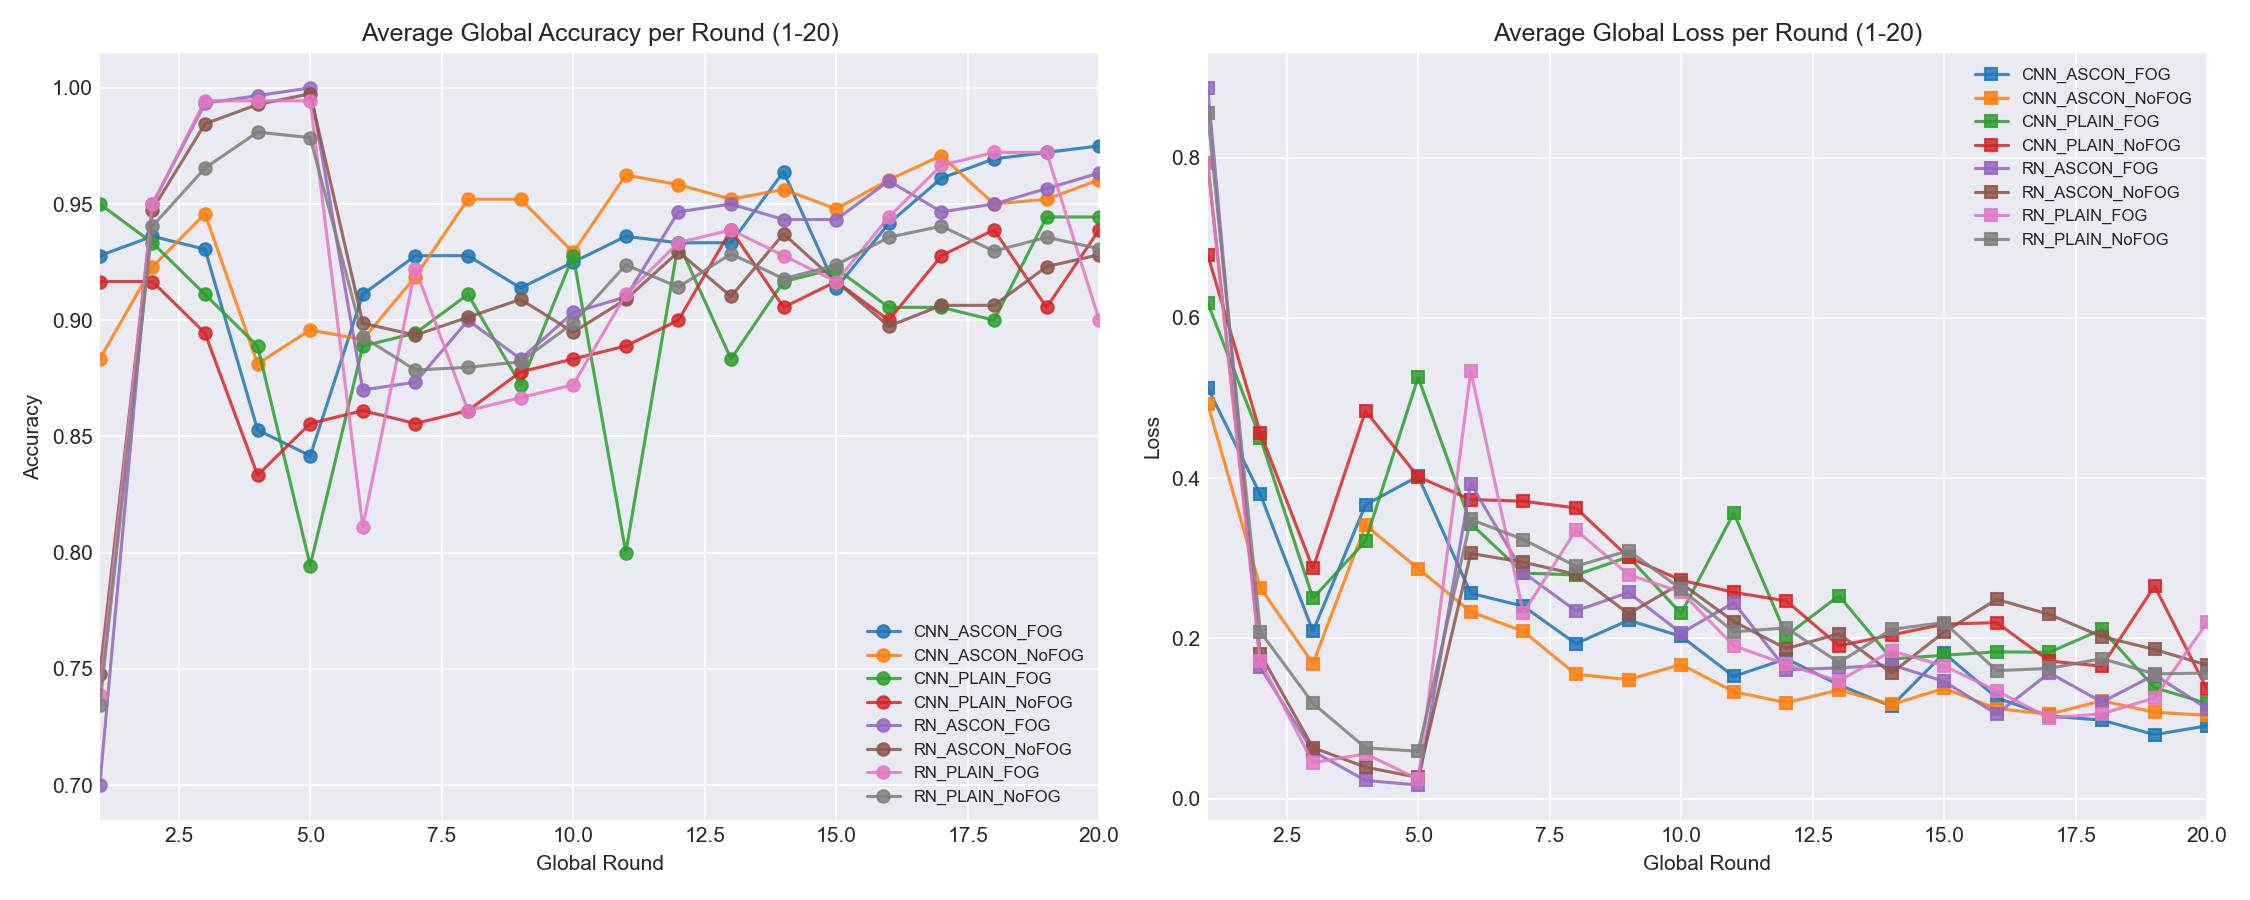
\includegraphics[width=\textwidth]{Figures/convergence_English.png}
    \caption{Convergence of the collaborative learning process across the eight experimental scenarios. The evolution of global accuracy and cross-entropy loss demonstrates the progressive optimization of the global model during federated training.}
    \label{fig:convergence}
\end{figure*}

La convergencia del proceso de aprendizaje constituye una condición necesaria, pero no suficiente, para validar el entrenamiento colaborativo. También es necesario verificar que dicha convergencia sea consecuencia de una dinámica de optimización estable y no de un comportamiento numéricamente inestable. Con este propósito, la Figura~\ref{fig:stability} presenta la evolución temporal de pesos representativos de las capas federadas durante el entrenamiento. En todas las configuraciones evaluadas, los parámetros evolucionan de forma continua y permanecen acotados a lo largo de las rondas de comunicación, sin presentar oscilaciones abruptas ni tendencias divergentes. Aunque cada escenario sigue trayectorias particulares como consecuencia de las decisiones arquitectónicas evaluadas, todos preservan una dinámica de optimización estable, lo que confirma la robustez del mecanismo jerárquico de agregación implementado en la arquitectura propuesta.

\begin{figure*}[ht]
    \centering
    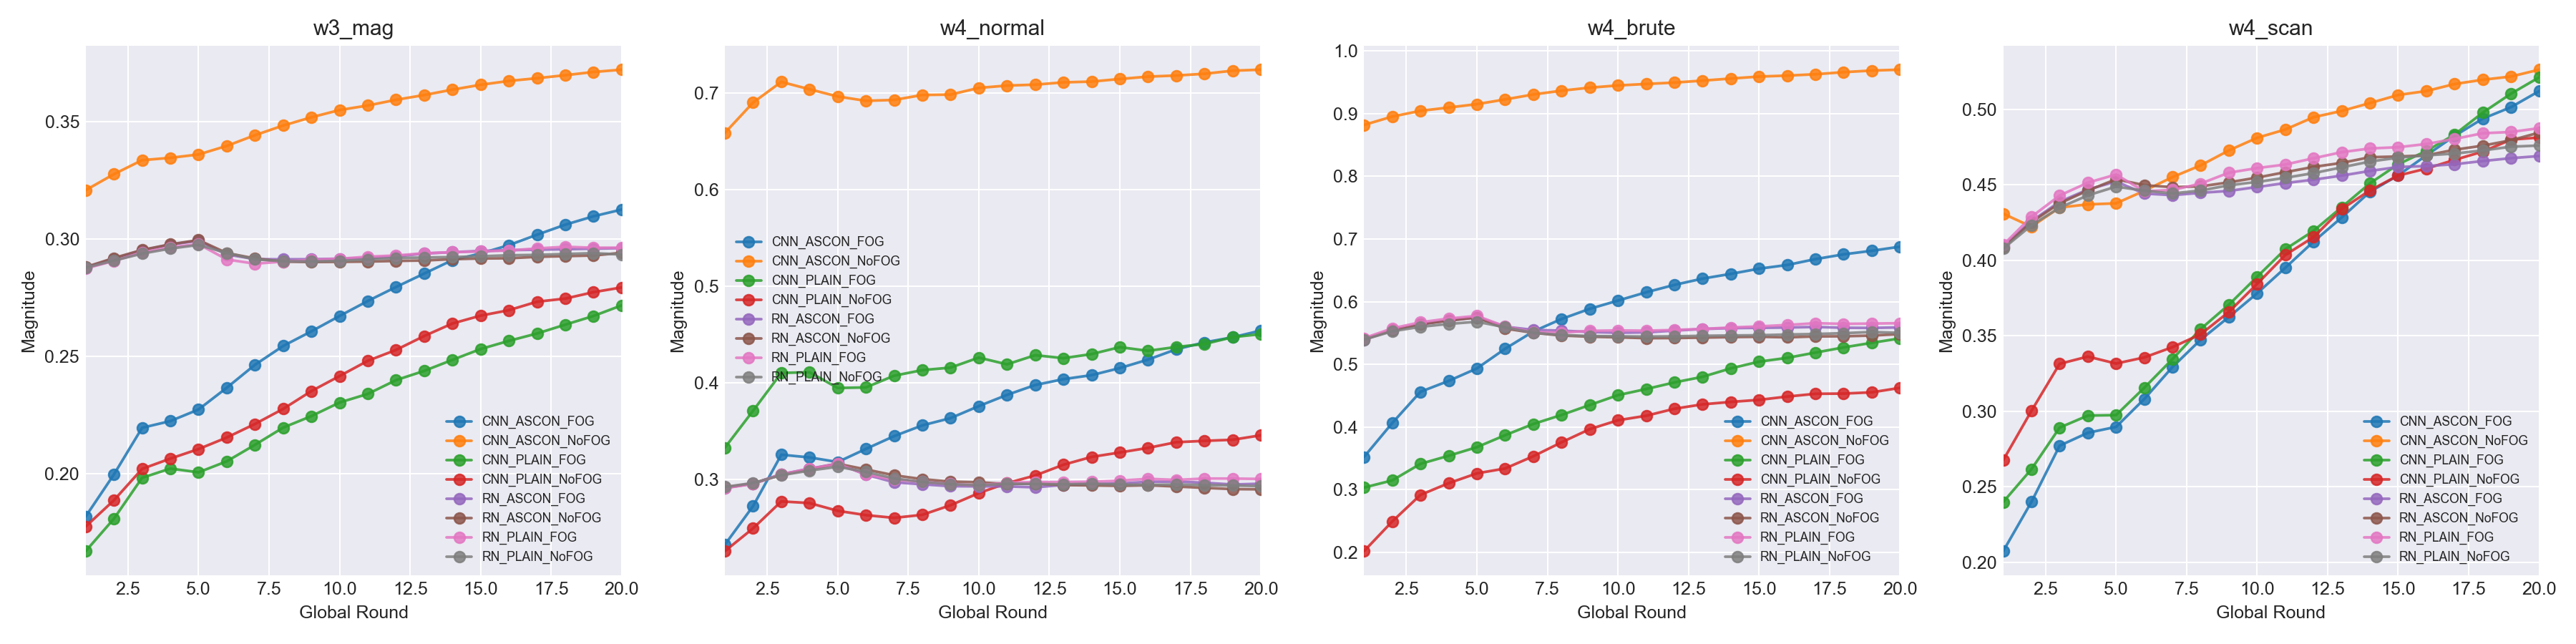
\includegraphics[width=\textwidth]{Figures/Stability_English.png}
    \caption{Stability of the collaborative learning process across the eight experimental scenarios. The evolution of representative federated parameters indicates a stable optimization process, with no evidence of divergence during collaborative training.}
    \label{fig:stability}
\end{figure*}

Las dos evidencias anteriores validan el proceso de aprendizaje federado desde perspectivas complementarias. Mientras la convergencia demuestra que el entrenamiento distribuido mejora progresivamente el desempeño del modelo global, el análisis de estabilidad confirma que dicha convergencia se alcanza mediante una dinámica de optimización consistente durante todo el entrenamiento. En conjunto, ambas propiedades garantizan que las diferencias observadas posteriormente en la capacidad de detección, la eficiencia operacional y el impacto de la protección criptográfica responden al efecto de las decisiones arquitectónicas evaluadas y no a inestabilidades inherentes al proceso de aprendizaje.

En conjunto, la evidencia experimental demuestra que la estrategia de aprendizaje federado jerárquico implementada en la arquitectura propuesta permite construir un modelo global mediante un proceso de optimización estable y consistente bajo las diferentes configuraciones experimentales evaluadas. Esta validación confirma la confiabilidad del proceso de aprendizaje distribuido y establece la base para la siguiente subsección, donde se analiza si el modelo obtenido mediante este entrenamiento colaborativo preserva la capacidad de detección de la arquitectura propuesta.

\subsection{Capacidad de detección de la arquitectura propuesta}
Las subsecciones anteriores validaron que la arquitectura propuesta satisface las condiciones necesarias para implementar un sistema de aprendizaje colaborativo sobre dispositivos con recursos restringidos. En particular, se demostró que el modelo de inferencia seleccionado es compatible con las limitaciones del entorno \textit{Edge} y que el proceso de aprendizaje federado jerárquico converge mediante una dinámica de optimización estable. Una vez verificadas estas propiedades, el siguiente paso consiste en determinar si las decisiones arquitectónicas incorporadas durante el diseño preservan la funcionalidad principal del sistema como mecanismo de detección de intrusiones.

Desde una perspectiva arquitectónica, esta evaluación constituye la validación funcional de la propuesta. La incorporación de aprendizaje federado jerárquico, agregación multinivel y mecanismos criptográficos para proteger el intercambio de parámetros introduce nuevos procesos de coordinación que potencialmente podrían afectar el desempeño del sistema. En consecuencia, el objetivo de esta subsección es verificar que estas decisiones de diseño preservan la capacidad de distinguir entre tráfico legítimo y tráfico malicioso bajo las diferentes configuraciones experimentales consideradas.

La Tabla~\ref{tab:detection_capability} resume el desempeño de clasificación obtenido para las ocho configuraciones experimentales evaluadas. La comparación integra las principales métricas empleadas para caracterizar sistemas de detección de intrusiones y permite analizar el efecto conjunto del modelo de inferencia, de la arquitectura de agregación y del mecanismo de protección de las comunicaciones sobre el comportamiento funcional del sistema.

\begin{table*}[ht]
\centering
\caption{Detection performance obtained for the eight experimental configurations evaluated in the proposed architecture.}
\label{tab:detection_capability}
\footnotesize
\begin{tabular}{lccccccc}
\toprule
&
\multicolumn{3}{c}{\textbf{Experimental Configuration}}
&
\multicolumn{4}{c}{\textbf{Detection Performance}}
\\
\cmidrule(lr){2-4}
\cmidrule(lr){5-8}
\textbf{Scenario} & \textbf{Inference Model} &  \textbf{Architecture} & \textbf{Protection} & \textbf{Accuracy\textsuperscript{a}} & \textbf{Precision\textsuperscript{b}} & \textbf{Recall\textsuperscript{b}} & \textbf{F1-score\textsuperscript{b}}
\\
\midrule
E1 & MLP & Edge--Cloud      & ASCON & 93.81 & 92.11 & 90.72 & 90.82 \\
E2 & MLP & Edge--Cloud      & PLAIN & 92.98 & 92.11 & 90.72 & 90.82 \\
E3 & MLP & Edge--Fog--Cloud & ASCON & 96.33 & 92.11 & 90.72 & 90.82 \\
E4 & MLP & Edge--Fog--Cloud & PLAIN & 90.00 & 92.11 & 90.72 & 90.82 \\
E5 & CNN & Edge--Cloud      & ASCON & 96.04 & 92.09 & 90.70 & 90.80 \\
E6 & CNN & Edge--Cloud      & PLAIN & 93.89 & 92.09 & 90.70 & 90.80 \\
E7 & CNN & Edge--Fog--Cloud & ASCON & 97.50 & 92.09 & 90.70 & 90.80 \\
E8 & CNN & Edge--Fog--Cloud & PLAIN & 94.44 & 92.09 & 90.70 & 90.80 \\
\bottomrule
\end{tabular}
\vspace{2mm}
\begin{flushleft}
\footnotesize\textit{Note:} All values in \%. \textsuperscript{a}~Accuracy is the mean final global accuracy measured on-device across the federated runs of each scenario (58 runs). \textsuperscript{b}~Precision, Recall and F1-score (weighted) are computed offline on the held-out 20\% stratified test set (51{,}255 flows) using the deployed MLP and CNN-1D models, since the federated runtime logged only global accuracy and loss; therefore these three metrics depend on the inference model and are shared by its four scenarios.
\end{flushleft}
\end{table*}

La evidencia experimental permite analizar el efecto conjunto de las principales decisiones arquitectónicas incorporadas durante el diseño. En primer lugar, la comparación entre los modelos de inferencia MLP y CNN permite verificar si la selección de la arquitectura TinyML influye sobre la capacidad de detección alcanzada por el sistema. En segundo lugar, la evaluación de las arquitecturas \textit{Edge--Cloud} y \textit{Edge--Fog--Cloud} permite determinar si la incorporación de un nivel intermedio de agregación modifica el desempeño del modelo global. Finalmente, la comparación entre las configuraciones protegidas mediante ASCON y aquellas que utilizan comunicaciones sin protección permite establecer si la protección criptográfica del proceso de aprendizaje federado introduce alguna degradación en las métricas de clasificación.

Los resultados resumidos en la Tabla~\ref{tab:detection_capability} muestran que ninguno de los tres factores compromete la capacidad de detección del sistema. En cuanto al modelo de inferencia, las configuraciones basadas en CNN alcanzan una exactitud promedio del 95.5\%, ligeramente superior a la obtenida por las variantes MLP (93.3\%), lo que confirma que ambas arquitecturas TinyML preservan un desempeño equivalente pese a su diferente complejidad. Respecto a la topología de aprendizaje, la incorporación de la capa \textit{Fog} produce un efecto favorable pero no uniforme: mejora la exactitud en las configuraciones protegidas con ASCON (+2.5 puntos en MLP y +1.5 en CNN) y en CNN sin protección (+0.6 puntos), mientras que en la combinación MLP sin protección introduce una ligera reducción (\(-3.0\) puntos), lo que indica que el beneficio de la agregación intermedia depende de la estabilidad de los mensajes intercambiados. Finalmente, la comparación entre configuraciones protegidas y no protegidas muestra que la incorporación de ASCON no degrada el desempeño: en las cuatro parejas equivalentes, las variantes con ASCON igualan o superan a sus contrapartes PLAIN, con diferencias de entre +0.8 y +6.3 puntos de exactitud. No obstante, este resultado debe interpretarse con cautela, ya que la evaluación no incluyó escenarios con fallos o mensajes corruptos inducidos; por lo tanto, la evidencia permite afirmar que la protección criptográfica es compatible con el proceso de aprendizaje, pero no que lo mejore de manera intrínseca. Los valores de \textit{precision}, \textit{recall} y \textit{F1-score}, determinados por el modelo de inferencia desplegado, permanecen prácticamente constantes (\(\approx\)90.8\% de \textit{F1-score} ponderado en ambas arquitecturas), lo que refuerza la homogeneidad del comportamiento de clasificación entre configuraciones.

Más allá del efecto individual de cada decisión de diseño, el aspecto más relevante corresponde al comportamiento global de la arquitectura. Las ocho configuraciones evaluadas mantienen una exactitud comprendida entre el 90.0\% (E4, MLP--\textit{Edge--Fog--Cloud}--PLAIN) y el 97.5\% (E7, CNN--\textit{Edge--Fog--Cloud}--ASCON), lo que sitúa la totalidad de las variantes por encima del umbral del 90\% y acota la variación máxima a 7.5 puntos porcentuales. Esta dispersión, limitada y sin ninguna configuración que colapse el desempeño, demuestra que la capacidad de detección se preserva de forma consistente en todo el espacio de diseño explorado. La mejor combinación (CNN con agregación \textit{Fog} y protección ASCON) y la más modesta difieren únicamente en la elección conjunta del modelo, la topología y el mecanismo de protección, sin que ninguna de estas decisiones, por sí sola, reduzca la exactitud por debajo del rango operativo. En consecuencia, la capacidad de detección constituye una propiedad robusta de la arquitectura propuesta y no depende exclusivamente de una combinación particular del modelo de inferencia, de la estrategia de agregación o del mecanismo de protección utilizado.

En conjunto, esta evaluación completa la validación funcional de la arquitectura propuesta. Las subsecciones anteriores demostraron la viabilidad del despliegue sobre dispositivos \textit{Edge} y la estabilidad del proceso de aprendizaje federado jerárquico, mientras que la presente subsección verifica que dichas decisiones de diseño preservan la capacidad de detección del sistema. Esta validación establece el punto de partida para analizar, en la siguiente subsección, el costo operacional asociado a las principales decisiones arquitectónicas implementadas.

\subsection{Eficiencia operacional de la arquitectura propuesta}

Una vez validada la capacidad de detección del sistema, el siguiente paso consiste en evaluar su eficiencia operacional. Esta evaluación determina si el aprendizaje federado jerárquico y la protección criptográfica de las comunicaciones pueden integrarse manteniendo un comportamiento temporal estable y un costo compatible con la operación continua de una infraestructura IoT distribuida.

La Figura~\ref{fig:round_duration} muestra la evolución del tiempo promedio requerido para completar cada ronda de aprendizaje durante las veinte iteraciones del proceso federado para las ocho configuraciones experimentales evaluadas.

\begin{figure*}[ht]
    \centering
    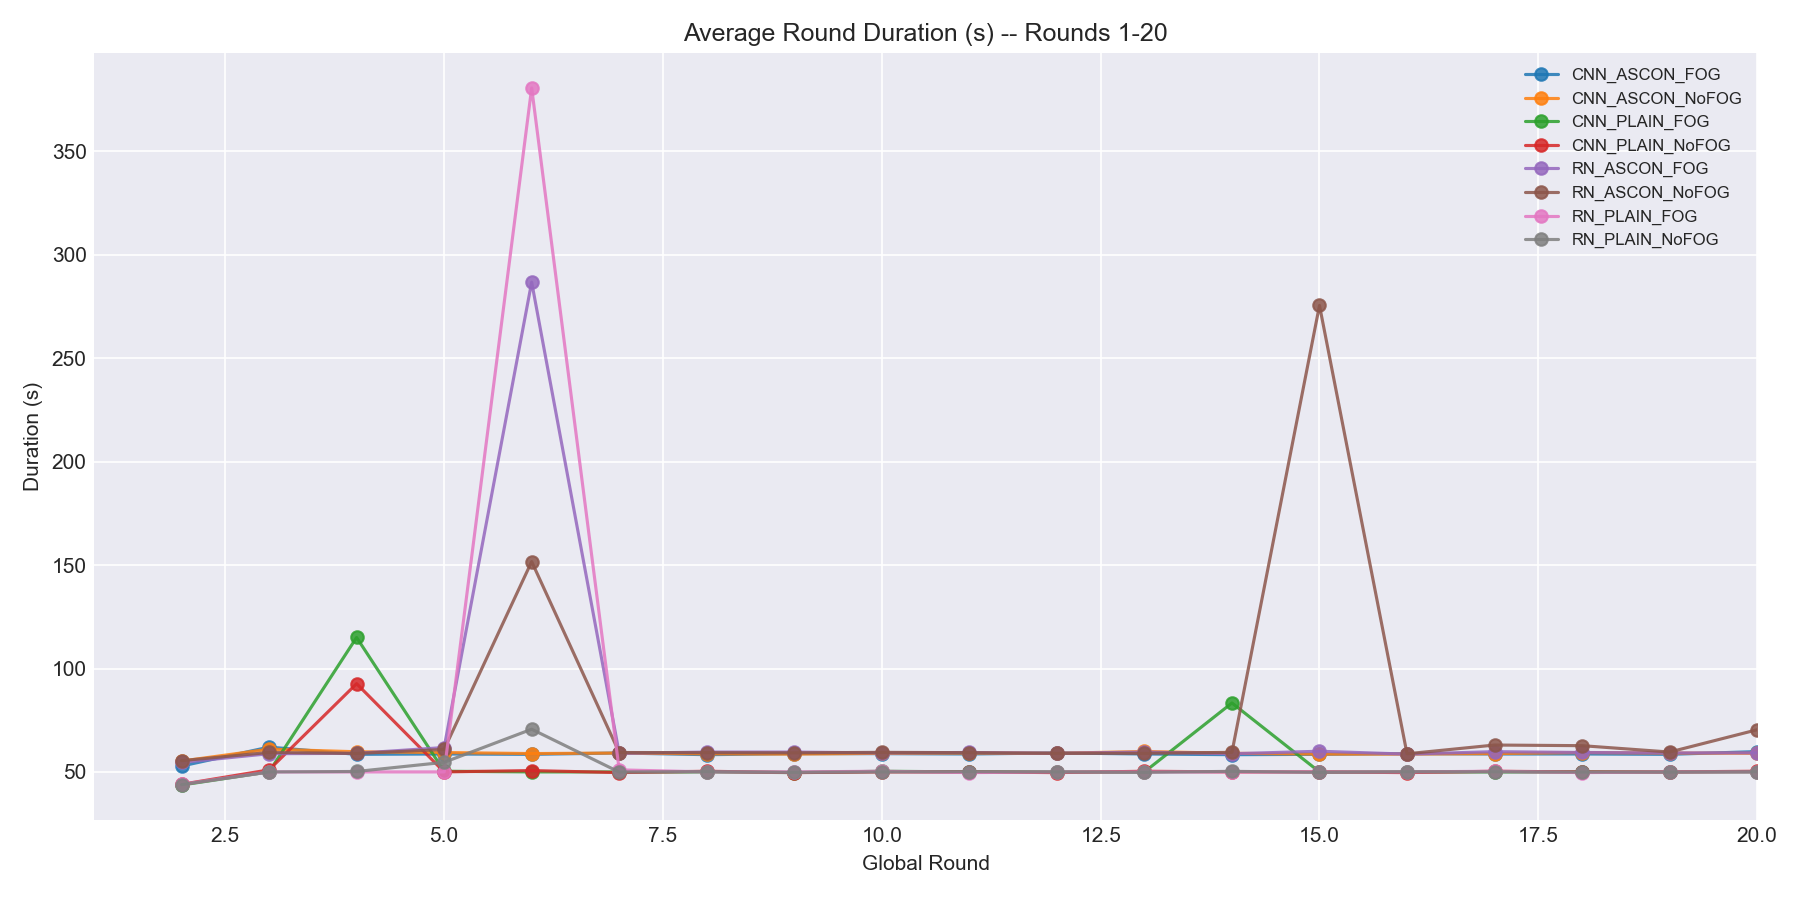
\includegraphics[width=\textwidth]{Figures/Round_Duration_English.png}
    \caption{Average duration of each federated learning round across the eight experimental configurations.}
    \label{fig:round_duration}
\end{figure*}

La Tabla~\ref{tab:training_time} resume el tiempo promedio requerido para completar una ronda de aprendizaje en cada configuración experimental.

\begin{table}[ht]
\centering
\caption{Average time required to complete one federated learning round.}
\label{tab:training_time}
\footnotesize
\begin{tabular}{lc}
\toprule
\textbf{Configuration} & \textbf{Time per Round (s)} \\
\midrule
CNN + ASCON + Fog      & 58.61 \\
CNN + ASCON + NoFog    & 58.97 \\
CNN + Plain + Fog      & 54.86 \\
CNN + Plain + NoFog    & 52.02 \\
MLP + ASCON + Fog      & 71.13 \\
MLP + ASCON + NoFog    & 72.91 \\
MLP + Plain + Fog      & 67.14 \\
MLP + Plain + NoFog    & 51.01 \\
\midrule
\textbf{Overall Average} & \textbf{61.36} \\
\bottomrule
\end{tabular}
\end{table}

La evolución temporal evidencia un comportamiento consistente en todas las configuraciones evaluadas. Después de las primeras rondas de entrenamiento, el tiempo requerido para completar cada iteración converge hacia un régimen prácticamente estacionario, manteniéndose alrededor de un valor constante durante el resto del proceso de aprendizaje. No se observa un incremento progresivo en la duración de las rondas, lo que indica que el sistema mantiene un costo operacional estable aun cuando incorpora múltiples niveles de agregación y coordinación distribuida.

Los tiempos promedio obtenidos muestran que las diferentes configuraciones experimentales requieren entre 51.01 y 72.91 segundos para completar una ronda de aprendizaje, con un promedio global de 61.36 segundos. Aunque las distintas combinaciones del modelo de inferencia, la estrategia de agregación y el mecanismo de protección modifican el tiempo absoluto requerido por cada configuración, todas preservan un comportamiento temporal consistente durante el entrenamiento. Desde una perspectiva de ingeniería, esta estabilidad permite anticipar el costo asociado a cada ciclo de aprendizaje, facilitando la planificación de las actualizaciones del modelo global y la asignación de recursos computacionales en infraestructuras IoT distribuidas.

Además del costo asociado al entrenamiento distribuido, la eficiencia operacional también depende de la protección criptográfica aplicada al intercambio de parámetros entre los diferentes niveles del sistema. Por esta razón, el siguiente análisis caracteriza la sobrecarga computacional y de comunicación introducida por ASCON durante el proceso de aprendizaje federado.

La Figura~\ref{fig:crypto_latency} muestra la latencia p95 medida para las principales operaciones criptográficas realizadas durante el intercambio de parámetros entre los distintos niveles de la arquitectura.

\begin{figure*}[ht]
    \centering
    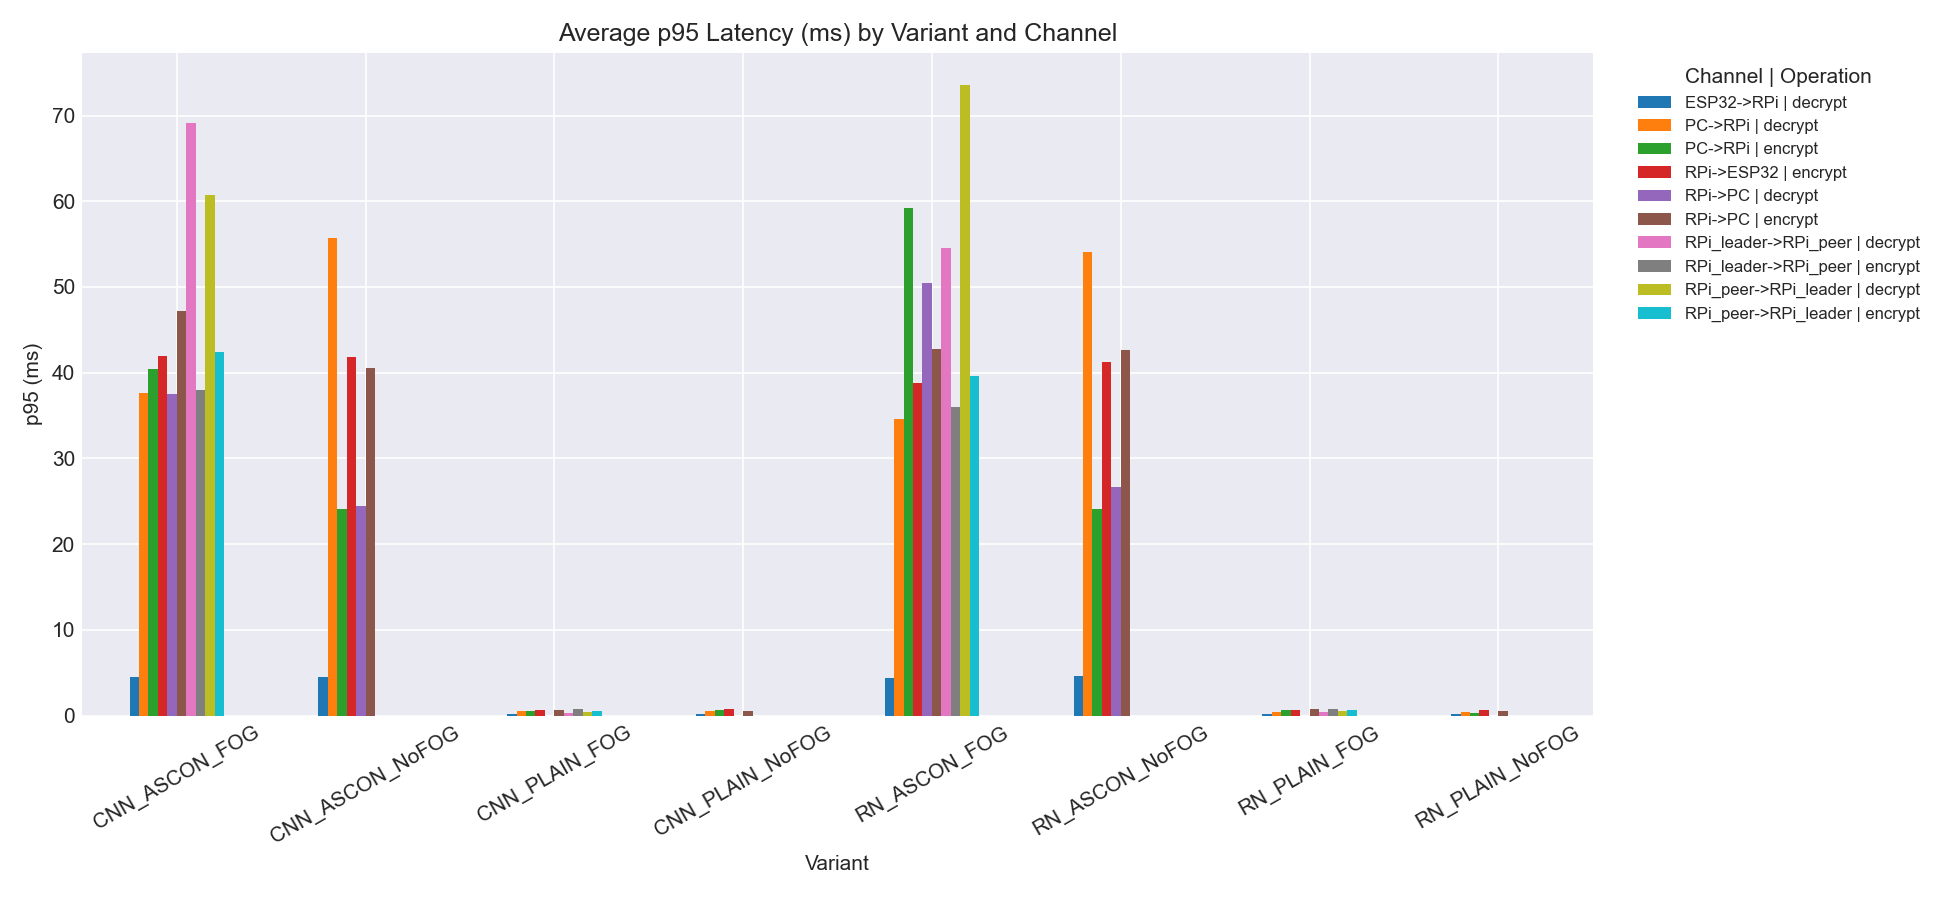
\includegraphics[width=\textwidth]{Figures/Crypto_Latency_English.png}
    \caption{p95 latency of cryptographic operations across the communication channels of the proposed architecture.}
    \label{fig:crypto_latency}
\end{figure*}

La Tabla~\ref{tab:crypto_latency} resume las latencias promedio observadas en las principales operaciones criptográficas.

\begin{table}[ht]
\centering
\caption{Average p95 latency (ms) of the main cryptographic operations.}
\label{tab:crypto_latency}
\footnotesize
\begin{tabular}{lccc}
\toprule
\textbf{Configuration} & \textbf{ESP32$\rightarrow$RPi} & \textbf{RPi$\rightarrow$PC} & \textbf{PC$\rightarrow$RPi} \\
\midrule
CNN + ASCON + Fog      & 4.53 & 37.47 & 40.37 \\
CNN + ASCON + NoFog    & 4.55 & 24.46 & 24.12 \\
MLP + ASCON + Fog      & 4.37 & 50.47 & 59.18 \\
MLP + ASCON + NoFog    & 4.65 & 26.69 & 24.14 \\
\bottomrule
\end{tabular}
\end{table}

La evidencia experimental demuestra que el costo criptográfico se distribuye de forma jerárquica a lo largo de la arquitectura. Las operaciones realizadas sobre los dispositivos \textit{Edge} presentan latencias reducidas y prácticamente constantes entre configuraciones, mientras que los mayores tiempos se concentran en las comunicaciones entre los niveles \textit{Fog} y \textit{Cloud}. Esta distribución resulta consistente con el diseño propuesto, donde los nodos intermedios procesan un mayor volumen de información y disponen simultáneamente de mayores capacidades computacionales para absorber el costo asociado a la protección de las comunicaciones. Las latencias reportadas representan únicamente el tiempo asociado a las operaciones criptográficas y constituyen una fracción del tiempo total requerido para completar una ronda de aprendizaje.

El segundo componente de la eficiencia operacional corresponde al costo de comunicación introducido por la protección criptográfica. La Figura~\ref{fig:payload_overhead} muestra el tamaño promedio de los mensajes transmitidos en cada canal de comunicación y el \textit{overhead} adicional generado por el mecanismo de protección.

\begin{figure*}[ht]
    \centering
    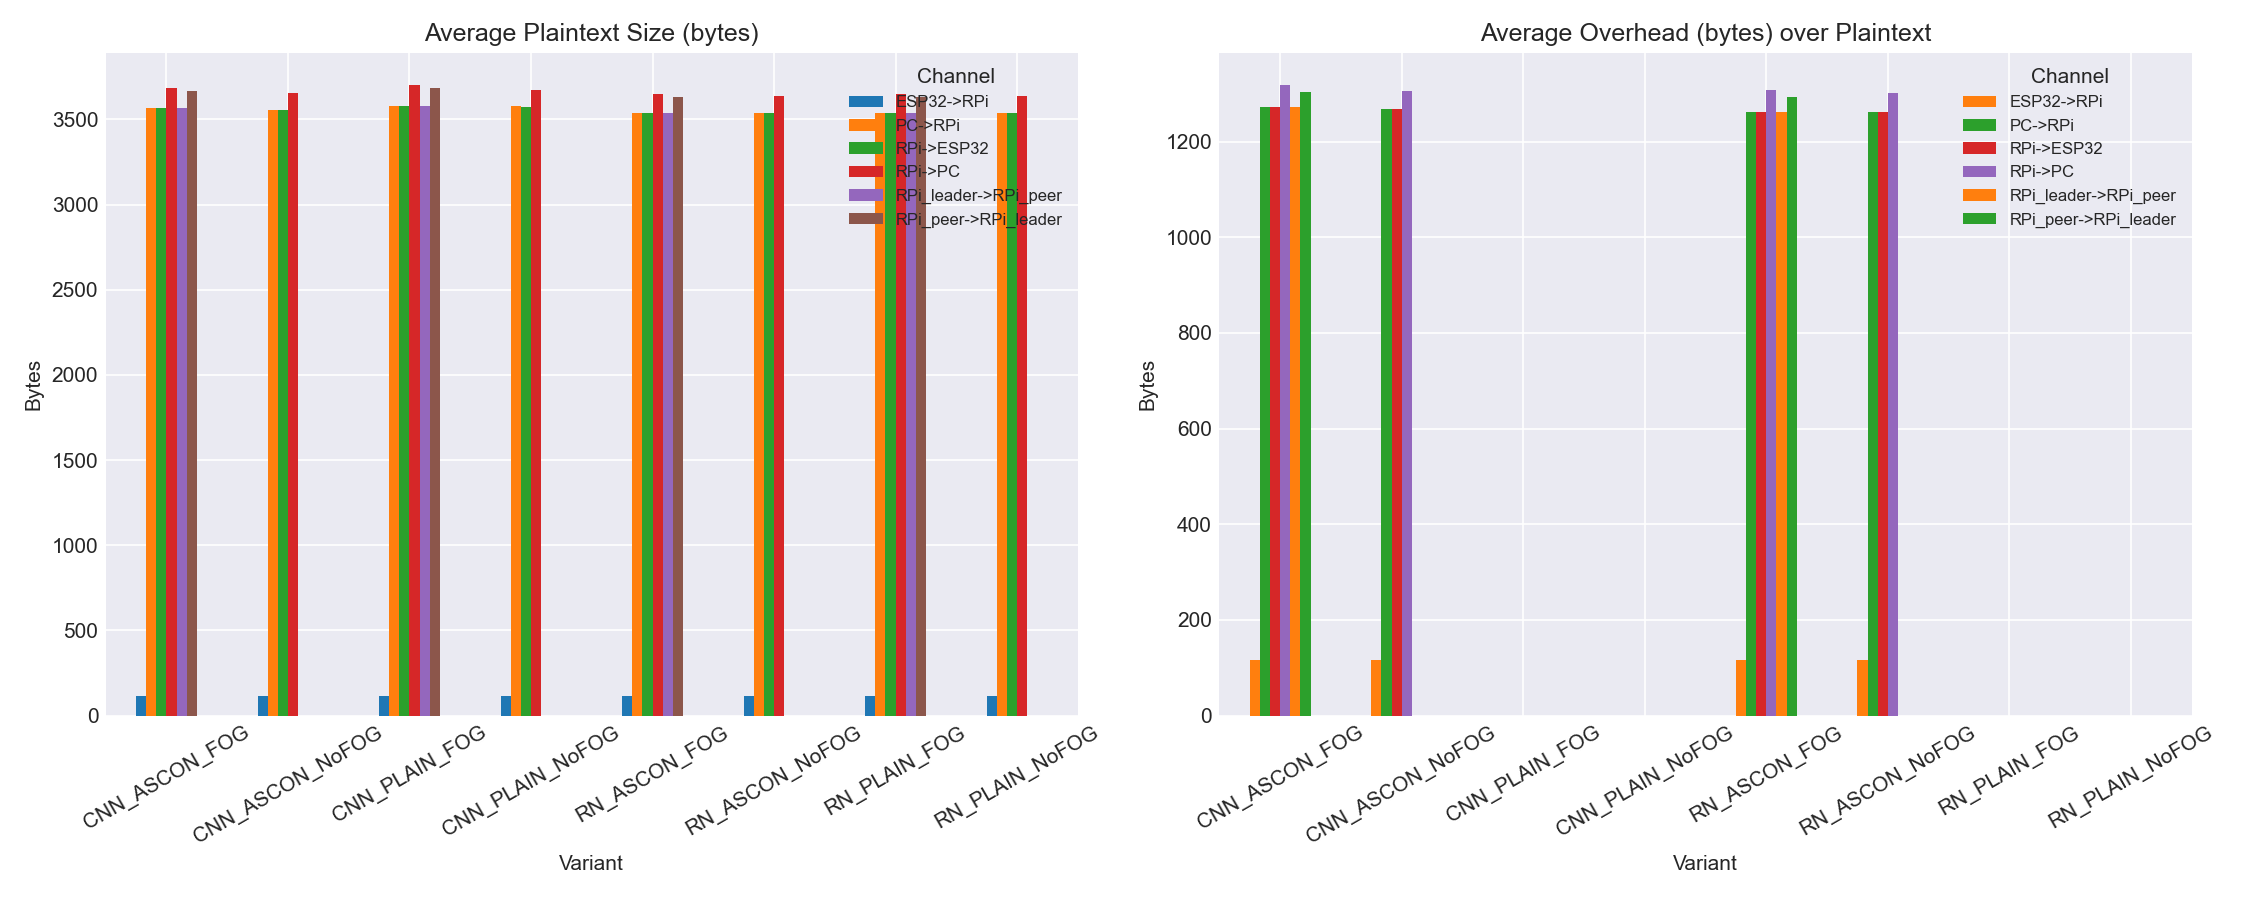
\includegraphics[width=\textwidth]{Figures/Payload_Overhead_English.png}
    \caption{Average payload size by communication channel: plaintext payload (left) and additional overhead introduced by the cryptographic mechanism (right).}
    \label{fig:payload_overhead}
\end{figure*}

La Tabla~\ref{tab:payload_overhead} resume el tamaño promedio de los mensajes protegidos y el \textit{overhead} introducido por el mecanismo criptográfico.

\begin{table}[ht]
\centering
\caption{Average communication overhead introduced by the cryptographic protection mechanism.}
\label{tab:payload_overhead}
\footnotesize
\begin{tabular}{lccc}
\toprule
\textbf{Configuration} & \textbf{Plaintext (B)} & \textbf{Overhead (B)} & \textbf{Ratio (\%)} \\
\midrule
CNN + ASCON + Fog      & 2365 & 1098 & 46.46 \\
CNN + ASCON + NoFog    & 2143 & 1049 & 48.94 \\
MLP + ASCON + Fog      & 2323 & 1084 & 46.64 \\
MLP + ASCON + NoFog    & 2162 & 1050 & 48.55 \\
\midrule
\textbf{Average} & \textbf{2248} & \textbf{1070} & \textbf{47.65} \\
\bottomrule
\end{tabular}
\end{table}

Los resultados muestran que el volumen de información intercambiado permanece prácticamente constante entre las distintas configuraciones evaluadas. Independientemente del modelo de inferencia o de la incorporación de la capa \textit{Fog}, los mensajes mantienen tamaños similares en un mismo canal de comunicación. En promedio, la protección criptográfica añade aproximadamente 1070 bytes a un \textit{payload} original de 2248 bytes, lo que representa un incremento cercano al 48\% del tamaño del mensaje. Aunque este incremento constituye un costo inherente al mecanismo de autenticación y confidencialidad implementado, su magnitud permanece prácticamente constante en todas las configuraciones evaluadas, permitiendo estimar de manera predecible el impacto de la protección criptográfica durante el diseño y despliegue del sistema.

En conjunto, la evidencia experimental demuestra que la eficiencia operacional del sistema está determinada por dos componentes complementarios: el costo asociado al aprendizaje federado y la sobrecarga introducida por la protección criptográfica de las comunicaciones. Los resultados muestran que ambos presentan un comportamiento estable y predecible durante todo el proceso de aprendizaje. Mientras el entrenamiento mantiene una duración consistente entre rondas, el costo criptográfico se concentra principalmente en los niveles \textit{Fog} y \textit{Cloud} e introduce un incremento prácticamente constante en el volumen de información transmitida. En consecuencia, la arquitectura integra aprendizaje federado jerárquico y comunicaciones seguras sin comprometer la viabilidad del despliegue, la estabilidad del entrenamiento ni la capacidad de detección previamente demostradas. En conjunto con las evidencias presentadas en esta sección, estos resultados validan la arquitectura \textit{Edge--Fog--Cloud} propuesta como una solución viable para la detección distribuida de intrusiones en entornos IoT con restricciones de recursos.

%%%%%%%%%%%%%%%%%%%%%%%%%%%%%%%%%%%%%%%%%%
\section{Discusión}

Los resultados experimentales obtenidos en este trabajo demuestran la viabilidad de integrar inferencia TinyML, aprendizaje federado jerárquico y comunicaciones seguras dentro de una arquitectura distribuida \textit{Edge--Fog--Cloud} para sistemas de detección de intrusiones en entornos IoT. Más allá de validar el desempeño de cada uno de estos componentes, la evidencia obtenida permite analizar cómo las decisiones adoptadas durante el diseño de la arquitectura influyen en el comportamiento global del sistema y en el equilibrio entre capacidad de detección, estabilidad del aprendizaje, eficiencia operacional y protección de las comunicaciones.

Desde esta perspectiva, la discusión se centra en interpretar el significado de estos resultados desde un enfoque arquitectónico. En lugar de evaluar tecnologías individuales de forma aislada, el análisis considera cómo su integración permite responder simultáneamente a las restricciones computacionales, operacionales y de seguridad propias de los dispositivos IoT con recursos limitados. Este cambio de perspectiva desplaza el interés desde la optimización de componentes específicos hacia la comprensión de los principios de diseño que favorecen la construcción de arquitecturas distribuidas capaces de mantener un desempeño equilibrado bajo condiciones de operación reales.

Con este propósito, la discusión se desarrolla en tres dimensiones complementarias. En primer lugar, se analizan las implicaciones arquitectónicas derivadas de la evidencia experimental, identificando los principios de diseño que emergen de la interacción entre los diferentes componentes del sistema. Posteriormente, la propuesta se posiciona frente a las tendencias recientes del estado del arte para contextualizar su aporte dentro de la evolución de las arquitecturas distribuidas para detección de intrusiones. Finalmente, se examinan las principales limitaciones del estudio y se discuten las oportunidades de investigación que pueden ampliar el alcance de la arquitectura en escenarios IoT de mayor escala y complejidad.

\subsection{Implicaciones arquitectónicas de la propuesta}
La evidencia experimental obtenida permite interpretar la arquitectura propuesta desde una perspectiva que trasciende la evaluación individual de sus componentes. Aunque la inferencia TinyML, el aprendizaje federado jerárquico y las comunicaciones seguras fueron analizados mediante experimentos específicos, su comportamiento no puede comprenderse de manera aislada. Los resultados indican que la viabilidad del sistema depende de la interacción entre estas decisiones de diseño, cuya integración permite responder simultáneamente a las restricciones computacionales, operacionales y de seguridad propias de los entornos IoT.

La evaluación del modelo de inferencia pone de manifiesto que las restricciones impuestas por los dispositivos \textit{Edge} deben incorporarse como un criterio de diseño desde las primeras etapas del desarrollo y no considerarse únicamente como una limitación del despliegue. La comparación entre los modelos evaluados evidencia que maximizar el desempeño predictivo no garantiza una solución viable cuando existen restricciones de memoria, capacidad de procesamiento y latencia. En contraste, los modelos diseñados para plataformas con recursos limitados logran preservar una elevada capacidad de detección sin comprometer la ejecución sobre el hardware objetivo: las ocho configuraciones evaluadas se mantuvieron por encima del 90\% de exactitud, con una variación máxima de 7.5 puntos porcentuales y el mejor desempeño en la combinación de CNN, agregación \textit{Fog} y protección ASCON. Esta observación refuerza la necesidad de concebir el entorno de despliegue como un elemento que condiciona el diseño de la arquitectura desde su formulación inicial.

La evaluación del aprendizaje federado jerárquico complementa esta interpretación al mostrar que la estabilidad del proceso de entrenamiento constituye una propiedad de la arquitectura y no únicamente del algoritmo de aprendizaje. La convergencia consistente del modelo global y el comportamiento estable observado durante las sucesivas rondas de entrenamiento indican que la coordinación jerárquica puede incorporarse sin introducir degradaciones progresivas en el funcionamiento del sistema. En consecuencia, la estabilidad operacional adquiere un papel equivalente al desempeño predictivo como criterio para el diseño de arquitecturas distribuidas basadas en aprendizaje federado.

Una conclusión similar se obtiene a partir de la evaluación de las comunicaciones seguras. El comportamiento estable del costo criptográfico y del incremento del volumen de información transmitida demuestra que la protección de las comunicaciones puede planificarse desde el diseño de la arquitectura sin afectar significativamente el proceso de aprendizaje colaborativo. Asimismo, la distribución de la carga computacional hacia los niveles \textit{Fog} y \textit{Cloud} evidencia que es posible incorporar mecanismos criptográficos ligeros preservando las limitaciones propias de los dispositivos \textit{Edge}. En este contexto, la seguridad deja de entenderse como una funcionalidad adicional y pasa a consolidarse como una propiedad inherente de la arquitectura distribuida.

Consideradas de manera conjunta, estas observaciones muestran que el diseño de arquitecturas distribuidas para sistemas de detección de intrusiones en entornos IoT requiere abordar de forma integrada múltiples decisiones arquitectónicas interdependientes. La capacidad de detección, las restricciones impuestas por el hardware, la estabilidad del aprendizaje colaborativo y la protección de las comunicaciones no constituyen objetivos independientes, sino dimensiones cuyo equilibrio determina la viabilidad operacional del sistema. Desde esta perspectiva, la principal aportación de este trabajo consiste en demostrar experimentalmente que dicho equilibrio puede alcanzarse mediante una estrategia de integración arquitectónica coherente sobre una infraestructura \textit{Edge--Fog--Cloud}. Este principio de diseño proporciona una base conceptual para orientar el desarrollo y la evaluación de futuras arquitecturas distribuidas para sistemas de detección de intrusiones en entornos IoT.

\subsection{Contribución de la arquitectura frente al estado del arte}
Las implicaciones arquitectónicas discutidas en la subsección anterior adquieren mayor significado cuando se analizan en el contexto de la evolución reciente de los sistemas de detección de intrusiones para entornos IoT. La revisión de la literatura muestra una transición progresiva desde arquitecturas centralizadas hacia soluciones distribuidas que incorporan inferencia sobre dispositivos \textit{Edge}, aprendizaje federado y mecanismos de protección para preservar la privacidad de la información durante el entrenamiento colaborativo. Esta evolución responde a la necesidad de afrontar simultáneamente las limitaciones computacionales de los dispositivos IoT, la distribución geográfica de los datos y los crecientes requisitos de privacidad y escalabilidad.

Aunque estas capacidades representan avances importantes para el desarrollo de IDS distribuidos, la mayoría de los trabajos las aborda como líneas de investigación relativamente independientes. En consecuencia, resulta difícil establecer hasta qué punto su integración modifica el comportamiento global de una arquitectura o cuáles son las implicaciones derivadas de su interacción. Con el propósito de contextualizar esta observación, la Tabla~\ref{tab:sota_comparison} compara las principales capacidades arquitectónicas presentes en trabajos representativos de la literatura reciente.

\begin{table*}[ht]
\centering
\caption{Comparación de capacidades arquitectónicas entre trabajos representativos y la arquitectura propuesta.}
\label{tab:sota_comparison}
\footnotesize
\begin{tabular}{l c c c c c c}
\toprule
\textbf{Trabajo} & \textbf{IDS} & \textbf{TinyML -- Edge} & \textbf{FL} & \textbf{HFL} & \textbf{Comunicaciones Seguras} & \textbf{Hardware -- Edge real}
\\
\midrule
Hajj et al. \cite{Hajj2023}            & \checkmark & --          & \checkmark & --          & --          & --          \\
Chaurasia et al. \cite{Chaurasia2024}  & \checkmark & --          & \checkmark & --          & --          & --          \\
Ficco et al. \cite{Ficco2024}          & \checkmark & \checkmark  & \checkmark & --          & --          & \checkmark  \\
Roy et al. \cite{Roy2023}              & \checkmark & --          & \checkmark & --          & --          & --          \\
Tran et al. \cite{Tran2026}            & --          & \checkmark  & \checkmark & \checkmark  & \checkmark  & \checkmark  \\
Heydari \& Mahmoud \cite{Heydari2024}  & \checkmark & \checkmark  & --          & --          & --          & \checkmark  \\
Saravana Balaji et al. \cite{SaravanaBalaji2023} & \checkmark & \checkmark  & --          & --          & \checkmark  & \checkmark  \\
Alshammari \cite{Alshammari2026}       & \checkmark & --          & \checkmark & \checkmark  & \checkmark  & --          \\
\midrule
\textbf{Este trabajo} & \checkmark  & \checkmark & \checkmark & \checkmark & \checkmark & \checkmark \\
\bottomrule
\end{tabular}
\end{table*}

La comparación pone de manifiesto una tendencia consistente en la literatura reciente: las distintas capacidades necesarias para construir sistemas de detección de intrusiones distribuidos suelen desarrollarse de forma independiente. Algunos trabajos priorizan la ejecución eficiente de modelos TinyML sobre dispositivos con recursos limitados; otros se centran en el aprendizaje federado, la agregación jerárquica o la incorporación de mecanismos criptográficos para proteger las comunicaciones. El caso más cercano a la propuesta corresponde al trabajo de Alshammari \cite{Alshammari2026}, que integra detección de intrusiones, criptografía ligera ASCON y aprendizaje federado jerárquico; sin embargo, su validación se realiza sobre conjuntos de datos de referencia ejecutados en infraestructura convencional, sin desplegar el ciclo completo sobre microcontroladores reales. Aunque estas contribuciones han impulsado avances significativos en cada una de estas dimensiones, son menos frecuentes las propuestas que evalúan experimentalmente su integración dentro de una arquitectura distribuida implementada sobre hardware real.

Desde esta perspectiva, la aportación de este trabajo consiste en proporcionar evidencia experimental sobre la viabilidad de integrar inferencia TinyML, aprendizaje federado jerárquico y comunicaciones seguras dentro de una arquitectura \textit{Edge--Fog--Cloud}. Más que optimizar alguno de estos componentes de forma aislada, los resultados muestran que su integración permite mantener simultáneamente la capacidad de detección, la estabilidad del aprendizaje colaborativo, la viabilidad del despliegue sobre dispositivos con recursos limitados y la protección de las comunicaciones durante todo el proceso de entrenamiento.

Esta interpretación complementa el estado actual de la literatura al desplazar el foco desde la optimización individual de componentes hacia la evaluación de su integración arquitectónica. En este sentido, la evidencia presentada sugiere que el desarrollo de futuras arquitecturas distribuidas para sistemas de detección de intrusiones puede beneficiarse de enfoques que consideren conjuntamente las decisiones de inferencia, aprendizaje y protección de las comunicaciones como elementos interdependientes de un mismo sistema. Más que incorporar nuevas capacidades de manera incremental, el desafío consiste en comprender cómo su interacción condiciona el comportamiento global de la arquitectura y determina su viabilidad en escenarios IoT reales.

\subsection{Limitaciones del estudio y perspectivas de investigación}
Los resultados obtenidos demuestran la viabilidad de integrar inferencia TinyML, aprendizaje federado jerárquico y comunicaciones seguras dentro de una arquitectura distribuida para sistemas de detección de intrusiones en entornos IoT. Sin embargo, el alcance de estas conclusiones está condicionado por el contexto experimental definido para esta investigación. Como en cualquier estudio de validación experimental, las decisiones adoptadas durante el diseño de la plataforma de evaluación delimitan el dominio de aplicación de los resultados y, al mismo tiempo, identifican nuevas oportunidades para extender el trabajo hacia escenarios de mayor complejidad.

La validación se realizó sobre una infraestructura \textit{Edge--Fog--Cloud} implementada con dispositivos reales y capacidades computacionales diferenciadas. Este entorno permitió analizar de manera controlada la interacción entre los principales componentes del sistema y verificar la estabilidad del aprendizaje colaborativo, la capacidad de detección y el impacto de incorporar mecanismos de protección de las comunicaciones. No obstante, el estudio no consideró escenarios con un número elevado de clientes federados, dispositivos altamente heterogéneos o condiciones dinámicas de conectividad. La evaluación bajo estas condiciones constituye un paso necesario para caracterizar el comportamiento de la arquitectura en despliegues IoT de mayor escala y analizar su capacidad de adaptación frente a condiciones operacionales más variables.

Asimismo, el modelo de amenazas considerado durante la evaluación se centró en la protección del intercambio de parámetros mediante mecanismos criptográficos ligeros. En consecuencia, no se analizaron amenazas dirigidas al propio proceso de aprendizaje federado, como ataques de envenenamiento del modelo (\textit{model poisoning}), clientes bizantinos, ataques de inferencia o mecanismos avanzados de preservación de la privacidad, entre ellos la privacidad diferencial, la agregación segura y la computación segura multipartita \cite{Bunko2026}. La incorporación de estas capacidades representa una evolución natural de la arquitectura propuesta y resulta consistente con las líneas de investigación que actualmente orientan el desarrollo de sistemas de aprendizaje federado seguros y resilientes.

Finalmente, las conclusiones presentadas corresponden al conjunto de datos, la plataforma de hardware y la configuración experimental utilizados en esta investigación. La evaluación sobre diferentes dominios de aplicación, plataformas \textit{Edge} con capacidades computacionales diversas y configuraciones alternativas de aprendizaje federado permitirá analizar el grado de generalización de los principios arquitectónicos identificados y establecer el alcance de su aplicabilidad en otros escenarios IoT.

En conjunto, estas consideraciones ponen de manifiesto que el diseño de sistemas distribuidos de detección de intrusiones continúa siendo un problema multidimensional en el que convergen restricciones de procesamiento, comunicación, aprendizaje colaborativo y seguridad. Los resultados obtenidos en este trabajo muestran que estas dimensiones pueden abordarse de manera integrada dentro de una misma arquitectura, al tiempo que evidencian la necesidad de seguir incorporando mecanismos que fortalezcan su escalabilidad, resiliencia y preservación de la privacidad. En este sentido, las líneas de investigación identificadas no representan extensiones independientes de la propuesta, sino la evolución natural de los principios de integración arquitectónica discutidos en este trabajo y una base para el desarrollo de futuras arquitecturas distribuidas para sistemas de detección de intrusiones en entornos IoT.

%%%%%%%%%%%%%%%%%%%%%%%%%%%%%%%%%%%%%%%%%%
\section{Conclusiones}

Este trabajo presentó y evaluó una arquitectura distribuida \textit{Edge--Fog--Cloud} para sistemas de detección de intrusiones en entornos IoT que integra inferencia TinyML, aprendizaje federado jerárquico y comunicaciones seguras. La evaluación experimental demostró que estas capacidades pueden incorporarse de manera coherente preservando simultáneamente la capacidad de detección, la estabilidad del aprendizaje colaborativo y la viabilidad de su ejecución sobre dispositivos con recursos computacionales restringidos.

Los resultados obtenidos muestran que el comportamiento de este tipo de arquitecturas no depende exclusivamente del desempeño alcanzado por cada uno de sus componentes, sino de la interacción entre las decisiones de inferencia, aprendizaje y protección de las comunicaciones. Consideradas de manera conjunta, estas decisiones preservaron la capacidad de detección en todas las configuraciones experimentales, que se mantuvieron por encima del 90\% de exactitud, y evidenciaron que la interacción entre los componentes de la arquitectura resulta determinante para su desempeño global, como refleja el hecho de que la mejor combinación surja de la integración conjunta del modelo de inferencia, la topología de agregación y el mecanismo de protección, y no de la optimización aislada de ninguno de ellos.

La comparación con el estado del arte evidenció que estas capacidades suelen abordarse como líneas de investigación independientes. En este contexto, este trabajo aporta evidencia experimental sobre la viabilidad de integrarlas dentro de una única arquitectura distribuida implementada sobre hardware real, complementando la literatura existente desde una perspectiva centrada en la evaluación de la arquitectura como un sistema integrado.

Finalmente, las limitaciones identificadas durante la evaluación ponen de manifiesto la necesidad de extender este tipo de arquitecturas hacia escenarios de mayor escala, incorporando mecanismos adicionales de escalabilidad, resiliencia y preservación de la privacidad. En conjunto, los resultados obtenidos proporcionan una base experimental para orientar futuras investigaciones sobre arquitecturas distribuidas de detección de intrusiones en entornos IoT, favoreciendo el desarrollo de soluciones capaces de responder simultáneamente a los desafíos de procesamiento, aprendizaje colaborativo y seguridad.

%%%%%%%%%%%%%%%%%%%%%%%%%%%%%%%%%%%%%%%%%%
\vspace{6pt}

%%%%%%%%%%%%%%%%%%%%%%%%%%%%%%%%%%%%%%%%%%
\authorcontributions{Conceptualization, S.J., N.C., and C.L.-G.; methodology, S.J., N.C., and C.L.-G.; software, S.J. and N.C.; validation, S.J., N.C., and C.L.-G.; formal analysis, S.J., N.C., and C.L.-G.; investigation, S.J. and N.C.; data curation, S.J. and N.C.; visualization, S.J. and N.C.; writing---original draft preparation, S.J. and N.C.; writing---review and editing, S.J., N.C., and C.L.-G.; supervision, C.L.-G.; project administration, C.L.-G. All authors have read and agreed to the published version of the manuscript.
}

\funding{This research received no external funding.
}

\institutionalreview{Not applicable.}

\informedconsent{Not applicable.}

\dataavailability{The datasets analyzed during this study are publicly available from their original sources. The source code, trained models, experimental scripts, and configuration files developed for this work will be made publicly available through a public GitHub repository upon publication. An archived version of the repository will also be deposited in Zenodo to ensure long-term accessibility and reproducibility.}

\acknowledgments{The authors would like to thank the Systems and Computing Engineering Department at Universidad de los Andes for providing the research environment and computational infrastructure that supported this work.}

\conflictsofinterest{The authors declare no conflict of interest.}

%%%%%%%%%%%%%%%%%%%%%%%%%%%%%%%%%%%%%%%%%%
\abbreviations{Abbreviations}{%
The following abbreviations are used in this manuscript:\\

\noindent
\begin{tabular}{@{}l p{12cm}}
AEAD & Authenticated Encryption with Associated Data\\
ASCON & Authenticated Encryption Scheme Selected by the NIST Lightweight Cryptography Standardization Process\\
CNN & Convolutional Neural Network\\
FedAvg & Federated Averaging\\
FL & Federated Learning\\
HFL & Hierarchical Federated Learning\\
IDS & Intrusion Detection System\\
IoT & Internet of Things\\
MLP & Multilayer Perceptron\\
MQTT & Message Queuing Telemetry Transport\\
RPi & Raspberry Pi\\
TinyML & Tiny Machine Learning
\end{tabular}
}

%%%%%%%%%%%%%%%%%%%%%%%%%%%%%%%%%%%%%%%%%%
\reftitle{References}

%=====================================
% References, variant B: internal bibliography
%=====================================

% ACS format
\isAPAandChicago{}
{
\begin{thebibliography}{999}

\bibitem{Ni2024}
Ni, C.; Li, S. Machine Learning Enabled Industrial IoT Security: Challenges, Trends and Solutions. \emph{Journal of Industrial Information Integration} \textbf{2024}, \emph{38}, 100549.

\bibitem{Amanullah2020}
Amanullah, M.A.; Ariyaluran Habeeb, R.A.; Nasaruddin, F.H.; Gani, A.; Ahmed, E.; Mohamed Nainar, A.S.; Md Akim, N.; Imran, M. Deep Learning and Big Data Technologies for IoT Security. \emph{Computer Communications} \textbf{2020}, \emph{151}, 495--517.

\bibitem{Bagaa2020}
Bagaa, M.; Taleb, T.; Bernal Bernabe, J.; Skarmeta, A. A Machine Learning Security Framework for IoT Systems. \emph{IEEE Access} \textbf{2020}, \emph{8}, 114066--114077.

\bibitem{SaravanaBalaji2023}
Saravana Balaji, B.; Paja, W.; Antonijevic, M.; Stoean, C.; Bacanin, N.; Zivkovic, M. IoT Integrated Edge Platform for Secure Industrial Application with Deep Learning. \emph{Human-centric Computing and Information Sciences} \textbf{2023}, \emph{13}, 19.

\bibitem{Tekin2023}
Tekin, B.; et al.
Energy Consumption of On-Device Machine Learning Models for IoT Intrusion Detection. \emph{Internet of Things} \textbf{2023}, 100670.

\bibitem{Amuthadevi2025}
Amuthadevi, C.; Kavin, S.P.R.; Shrestha, A.; Yamini, N.R.S.; Sharma, D.K. TinyML-Based Intrusion Detection System for Sustainable IoT Security: A Novel Approach. \emph{Results in Engineering}
\textbf{2025}.

\bibitem{Dini2024}
Dini, P.; Diana, L.; Elhanashi, A.; Saponara, S. Overview of AI Models and Tools in Embedded IIoT Applications. \emph{Electronics} \textbf{2024}, \emph{13}, 2322.

\bibitem{Heydari2024}
Heydari, F.; Mahmoud, Q.H. Implementation of Lightweight Machine Learning-Based Intrusion Detection System on IoT Devices of Smart Homes. \emph{Future Internet} \textbf{2024}.

\bibitem{Ficco2024}
Ficco, M.; Guerriero, A.; Milite, E.; Palmieri, F.; Pietrantuono, R.; Russo, S. Federated Learning for IoT Devices: Enhancing TinyML with On-Board Training. \emph{Information Fusion} \textbf{2024}, \emph{104}, 102189.

\bibitem{Ramadan2025}
Ramadan, M.N.A.; Abdo, A.R.; Eldin, A.T. Federated Learning and TinyML on IoT Edge Devices: Current Practices, Limitations, and Open Challenges. \emph{Internet of Things} \textbf{2025}.

\bibitem{McMahan2017}
McMahan, B.; Moore, E.; Ramage, D.; Hampson, S.; Arcas, B.A.Y. Communication-Efficient Learning of Deep Networks from Decentralized Data. In \emph{Proceedings of the 20th International Conference on Artificial Intelligence and Statistics (AISTATS)}; PMLR, 2017; Vol.~54, pp.~1273--1282.

\bibitem{Imteaj2022}
Imteaj, A.; Thakker, U.; Wang, S.; Li, J.; Amini, M.H. A Survey on Federated Learning for Resource-Constrained IoT Devices. \emph{IEEE Internet of Things Journal} \textbf{2022}, \emph{9}, 1--24.

\bibitem{Hajj2023}
Hajj, S.; Azar, J.; Bou Abdo, J.; Demerjian, J.; Guyeux, C.; Makhoul, A.; Ginhac, D. Cross-Layer Federated Learning for Lightweight IoT Intrusion Detection Systems. \emph{Sensors} \textbf{2023}, \emph{23}, 7038.

\bibitem{Roy2023}
Roy, S.; Li, J.; Bai, Y. Federated Learning-Based Intrusion Detection System for IoT Environments with Locally Adapted Model. In \emph{Proceedings of the 2023 IEEE 10th International Conference on Cyber Security and Cloud Computing (CSCloud) / 2023 IEEE 9th International Conference on Edge Computing and Scalable Cloud (EdgeCom)}; IEEE, 2023; pp.~203--209.

\bibitem{Chaurasia2024}
Chaurasia, N.; Ram, M.; Verma, P.; Mehta, N.; Bharot, N. A Federated Learning Approach to Network Intrusion Detection Using Residual Networks in Industrial IoT Networks. \emph{The Journal of Supercomputing} \textbf{2024}, \emph{80}, 18325--18346.

\bibitem{Albanbay2025}
Albanbay, N.; Ajaei, F.B.; Shami, A. Federated Learning-Based Intrusion Detection in IoT Networks: Performance Evaluation and Data Scaling Study. \emph{Journal of Sensor and Actuator Networks} \textbf{2025}, \emph{14}, 78.

\bibitem{Tran2026}
Tran, T.-D.; Bui, P.-D.; Pham, V.-H. EdgeTrust-Shard: Hierarchical Blockchain Architecture for Federated Learning in Cross-Chain IoT Ecosystems. \emph{Journal of Systems Architecture} \textbf{2026}, \emph{173}, 103701.

\bibitem{NISTIR8454}
National Institute of Standards and Technology (NIST). NISTIR 8454: Lightweight Cryptography.
NIST Interagency/Internal Report (NISTIR), 2023. Available online: \url{https://csrc.nist.gov/pubs/ir/8454/final} (accessed on 7 February 2026).

\bibitem{NIST800232}
National Institute of Standards and Technology (NIST). Ascon-Based Lightweight Cryptography Standards for Constrained Devices: Authenticated Encryption, Hash, and Extendable Output Functions.
NIST Special Publication 800-232, 2025. Available online: \url{https://nvlpubs.nist.gov/nistpubs/SpecialPublications/NIST.SP.800-232.pdf}

\bibitem{Kaur2025}
Kaur, J.; Cintas-Canto, A.; Mozaffari-Kermani, M.; Azarderakhsh, R. A Survey on the Implementations, Attacks, and Countermeasures of the NIST Lightweight Cryptography Standard: ASCON. \emph{ACM Computing Surveys} \textbf{2025}, \emph{58}, 6:1--6:16.

\bibitem{Gusita2025}
Gusita, F.; Rahimi, S.; et al. Lightweight Cryptography for Internet of Things Devices: A Survey.
\emph{Jurnal Ilmiah Teknik Elektro Komputer dan Informatika (JITEKI)} \textbf{2025}, \emph{11}, 153--170.

\bibitem{Mirzaali2025}
Mirzaali, I.; Javadi, A.; Sadeghi, S.; Pahlevani, P.; Bagheri, N.; Bendavid, Y.; Rostampour, S. Evaluating Security Pitfalls of Ultra-Lightweight IoT Authentication: A Critical Analysis of Permutation Functions. \emph{Journal of Information Security and Applications} \textbf{2025}, \emph{93}, 104188.

\bibitem{Wang2019}
Wang, P.; Yang, L.T.; Li, J.; Chen, J.; Hu, S. Data Fusion in Cyber-Physical-Social Systems: State-of-the-Art and Perspectives. \emph{Information Fusion} \textbf{2019}, \emph{51}, 42--57.

\bibitem{CICIoT2023}
Neto, E.C.; Dadkhah, S.; Ferreira, R.; Zohourian, A.; Lu, R.; Ghorbani, A.A. CICIoT2023: A Real-Time Dataset and Benchmark for Large-Scale Attacks in IoT Environment. \emph{Sensors} \textbf{2023}, \emph{23}, 5941.

\bibitem{Zouhri2024}
Zouhri, H.; Idri, A.; Ratnani, A. Evaluating the Impact of Filter-Based Feature Selection in Intrusion Detection Systems. \emph{International Journal of Information Security} \textbf{2024}, \emph{23}, 759--785.

\bibitem{Banbury2020}
Banbury, C.R.; Reddi, V.J.; Lam, M.; Fu, W.; Fazel, A.; Holleman, J.; et al. Benchmarking TinyML Systems: Challenges and Direction. \emph{arXiv} \textbf{2020}, arXiv:2003.04821.

\bibitem{Li2017}
Li, J.; Cheng, K.; Wang, S.; Morstatter, F.; Trevino, R.P.; Tang, J.; Liu, H. Feature Selection: A Data Perspective. \emph{ACM Computing Surveys} \textbf{2018}, \emph{50}, 94:1--94:45.

\bibitem{Moustafa2019}
Moustafa, N.; Turnbull, B.P.; Choo, K.-K.R. An Ensemble Intrusion Detection Technique Based on Proposed Statistical Flow Features for Protecting Network Traffic of Internet of Things. \emph{IEEE Internet of Things Journal} \textbf{2019}, \emph{6}, 4815--4830.

\bibitem{Warden2019}
Warden, P.; Situnayake, D. \emph{TinyML: Machine Learning with TensorFlow Lite on Arduino and Ultra-Low-Power Microcontrollers}; O'Reilly Media: Sebastopol, CA, USA, 2019.

% ---------------------------------------------------------------
% Referencias incorporadas durante la revisión bibliográfica
% (verificadas contra Crossref / arXiv)
% ---------------------------------------------------------------

\bibitem{Lim2025}
Lim, K.S.; Ooi, S.Y.; Sayeed, M.S.; Chew, Y.J.; Ahmad, N.M. Securing the Internet of Things: Systematic Insights into Architectures, Threats, and Defenses. \emph{Electronics} \textbf{2025}, \emph{14}, 3972.

\bibitem{Tamuka2026}
Tamuka, N.; Mathonsi, T.E.; Olwal, T.O.; Maswikaneng, S.; Muchenje, T.; Tshilongamulenzhe, T.M. Intrusion Detection in Fog Computing: A Systematic Review of Security Advances and Challenges. \emph{Computers} \textbf{2026}, \emph{15}, 169.

\bibitem{Alshammari2026}
Alshammari, A. A Unified Low-Carbon Cybersecurity Framework Integrating Energy-Efficient Intrusion Detection, Lightweight Cryptography, and Carbon-Aware Scheduling for Edge--Cloud Architectures. \emph{Scientific Reports} \textbf{2026}, \emph{16}, 10603.

\bibitem{HeydariSurvey2025}
Heydari, S.; Mahmoud, Q.H. Tiny Machine Learning and On-Device Inference: A Survey of Applications, Challenges, and Future Directions. \emph{Sensors} \textbf{2025}, \emph{25}, 3191.

\bibitem{Bartoli2025}
Bartoli, P.; Veronesi, C.; Giudici, A.; Siorpaes, D.; Trojaniello, D.; Zappa, F. Benchmarking Energy and Latency in TinyML: A Novel Method for Resource-Constrained AI. \emph{arXiv} \textbf{2025}, arXiv:2505.15622.

\bibitem{Dritsas2025}
Dritsas, E.; Trigka, M. Federated Learning for IoT: A Survey of Techniques, Challenges, and Applications. \emph{Journal of Sensor and Actuator Networks} \textbf{2025}, \emph{14}, 9.

\bibitem{Cooray2025}
Cooray, L.; Sendanayake, J.; Vithanaarachchi, P.; Priyadarshana, Y.H.P.P. Deep Federated Learning: A Systematic Review of Methods, Applications, and Challenges. \emph{Frontiers in Computer Science} \textbf{2025}, \emph{7}, 1617597.

\bibitem{Ma2024}
Ma, C.; Li, X.; Huang, B.; Li, G.; Li, F. Personalized Client-Edge-Cloud Hierarchical Federated Learning in Mobile Edge Computing. \emph{Journal of Cloud Computing} \textbf{2024}, \emph{13}, 161.

\bibitem{Sorescu2025}
Sorescu, T.-G.; Chiriac, V.-M.; Stoica, M.-A.; Comsa, C.-R.; Soroaga, I.-G.; Contac, A. Comparative Performance Analysis of Lightweight Cryptographic Algorithms on Resource-Constrained IoT Platforms. \emph{Sensors} \textbf{2025}, \emph{25}, 5887.

\bibitem{Fusco2025}
Fusco, P.; Montefusco, A.; Rimoli, G.P.; Palmieri, F.; Ficco, M. TinyML-Based Intrusion Detection System for Handling Class Imbalance in IoT-Edge Domain Using Siamese Neural Network on MCU. In \emph{Advanced Information Networking and Applications (AINA 2025)}; Lecture Notes on Data Engineering and Communications Technologies; Springer: Cham, Switzerland, 2025; pp.~389--402.

\bibitem{Sun2026}
Sun, Y.; Qin, Y.; Chen, W.; Zhao, W.; Sun, H. EPC-TinyAD: An Energy- and Privacy-Aware Compressed TinyML Framework for Reliable Industrial Anomaly Detection on Resource-Constrained Edge Devices. \emph{Electronics} \textbf{2026}, \emph{15}, 2879.

\bibitem{Ren2024}
Ren, H.; Anicic, D.; Li, X.; Runkler, T. On-Device Online Learning and Semantic Management of TinyML Systems. \emph{ACM Transactions on Embedded Computing Systems} \textbf{2024}, \emph{23}, 1--32.

\bibitem{Bunko2026}
Bunko, T.; Johnstone, M.N.; Yang, W.; Scott, B.A. A Survey of Privacy-Preserving Federated Learning for Intrusion Detection Systems. \emph{Artificial Intelligence Review} \textbf{2026}, \emph{59}, 125.

\end{thebibliography}
}

%%%%%%%%%%%%%%%%%%%%%%%%%%%%%%%%%%%%%%%%%%
\PublishersNote{}
\end{document}
